% Preamble ------------------------------------------------------------------------

\documentclass[11pt]{article}

 % Package Loads ------------------------------------------------------------------

 \usepackage[utf8]{inputenc}
 \usepackage[T1]{fontenc}
 \usepackage{lmodern}

 \usepackage[letterpaper, total={6.5in, 9in}, footnotesep=0.3in]{geometry}
 \usepackage[colorlinks=true, allcolors=blue]{hyperref}
 \usepackage{sidecap, caption}
 \usepackage{enumitem}
 \usepackage{csquotes}
 \usepackage{appendix}

 \usepackage{graphicx}
 \usepackage{float}
 \usepackage{units}
 \usepackage{amsmath,amsfonts,amssymb}
 \usepackage{gensymb}
 
 \usepackage{titlesec}
 \usepackage{titling}
 \usepackage{authblk}
 \usepackage[style=numeric]{biblatex}

 % Path ---------------------------------------------------------------------------

 \graphicspath{{assets/}}
 \addbibresource{bibliography.bib}

 % Set Global Font ----------------------------------------------------------------

 \renewcommand{\rmdefault}{lmss}

 % Title Elements -----------------------------------------------------------------
 

 \title{
    {\vspace{-1.5cm}}
    {\hspace{-2cm}}   
    {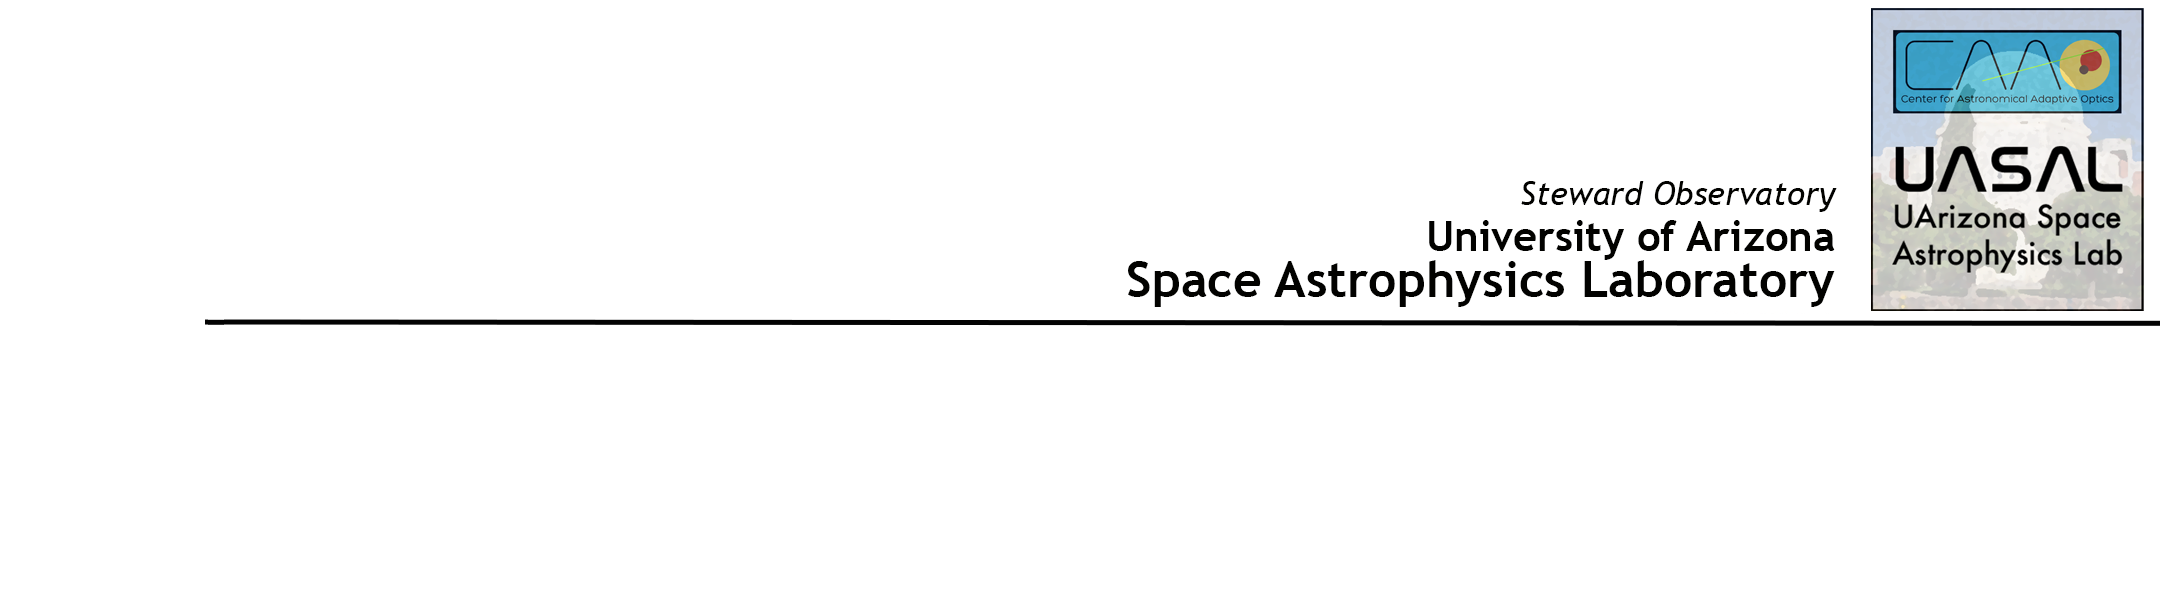
\includegraphics{assets/UASAL_Header.png}}
    {\large Comparison of}\\
    {Orbital Proton Fluences}\\
    {\Large \textit{For Typical Mission Orbits}}
 } 

 \author{\large Jess Johnson}

 \affil{\small Senior Instrumentation Scientist \\ Steward Observatory, University of Arizona \\ September 28, 2023}

 \date{}

% Document Start ------------------------------------------------------------------

\begin{document}

\fontfamily{lmss}
\maketitle

% Abstract ------------------------------------------------------------------------

\begin{abstract}
This paper compares proton fluxes for four typical mission orbits: the MEO orbit; the Molniya HEO orbit; the TESS P/2 HEO orbit, and the Spitzer Earth Trailing orbit (ETO); for more detail on individual orbits, see the Orbital Comparison memo. The proton fluences are the result of SPENVIS modeling, with the exception of the ETO, which is cited from Spitzer data. Illustrations of the orbital paths and their proximity to the Van Allen Radiation Belts are also presented.

\vspace{5mm}

\textit{\textbf{Author's note}: This memo has gone through substantial revision since its original posting. I have made a few tweaks to the P/2 HEO trajectory input in the SPENVIS orbit model, which corrected a geometry error in the original orbit. This has resulted in the P/2's fluence values to change considerably. I caught the mistake by realizing that the P/2 should not be generating significant trapped particle fluence as it lies completely outside the Van Allen belts. The values in this revision reflect this correction.} 

\end{abstract}

\newpage

% Table of Contents ---------------------------------------------------------------

\tableofcontents

\newpage

% Section One ---------------------------------------------------------------------

\section{Introduction}

This report shows proton Fluxes and fluences for several different orbits. In all but one case, these are the products of SPENVIS modeling; in the other, they are reproduced from other's work. and are credited as such. SPENVIS is designed to primarily address geocentric orbits; one of the orbits under consideration is a heliocentric orbit.

Although the scope of this paper is limited to high energy proton radiation, a few of the illustrations show the intersection of orbits with the Van Allen Belt electron regions; these are included without further data because the orbit's exposure to these regions warrant concern, and are obvious companion images to the proton region images. High energy electron fluxes and fluences will be addressed in an upcoming report.

Two sets of data for each orbit, excepting the heliocentric orbit, are presented. The first provides fluxes for trapped energetic protons, as well as proton fluences for a mission lifetime of one year. These were run with the standard NASA AP8 model set to simulate conditions of solar maxima. The second provide solar particle fluences under worst case scenarios. The sum of the two is a good representation of what should be the worst case situations for proton bombardment.

Finally, these fluxes and fluences do not take into account any form of shielding that the Pearl mission may implement. The point of this report is to show the radiation environment of individual orbits, so that exposure levels on different orbits can be compared.

\section{A few Notes}

\subsection{Reading the Simulation Output}

The SPENVIS flux and fluence tables are read as follows. Column one shows spectral energy bins. Column two shows the total mission \textit{flux}; i.e., the average, over the mission duration, of protons in this energy bin per centimeter squared per second. The third column shows the total mission \textit{fluence}; that is, the flux in this energy bin, integrated over the mission duration. Because these simulations were performed on the science trajectory only, there is only one mission segment, so the contents of columns four and five duplicate the contents of columns two and three. 

\subsection{Integral vs. Differential Spectra}

There are two different photon spectra types represented here. The first, the \textit{Integral Photon Spectrum}, represents the total number of photons emitted within a particular energy bin per unit time. It is a measure of the \textit{overall intensity} of the source within that bin's energy range. Its units are $\unit{/cm^2/s}$, or $\unit{/cm^2\cdot s}$. The second type, the \textit{Differential Photon Spectrum}, represents the rate of photon emission in a specific energy bin per unit energy, in this case, the MeV. It represents the \textit{energy distribution of the emitted photons}. Its units are $\unit{/cm^2/MeV/s}$, or $\unit{/cm^2\cdot MeV\cdot s}$. 

\subsection{Effects of Trapped Particle Radiation on Spacecraft Components}

The following is from the SPENVIS trapped particle radiation documentation. I reproduce it here because it is a concise statement of why the following results are critically important to orbit determination.\cite{website:spenvis01}

\begin{displayquote}
    \textbf{Effects of trapped particle radiation on spacecraft and components}

    Due to their large energy coverage, trapped particles cause a variety of effects in spacecraft, components and biological systems.
    
    Low energy electrons contribute to spacecraft surface charging. High energy electrons injected and accelerated through the magnetotail can cause dielectric charge buildup deep inside geosynchronous spacecraft which may lead in turn to destructive arcing. Inner and outer belt electrons also contribute to ionising doses through direct energy deposition and bremsstrahlung effects.

    High energy protons in the inner radiation belt are the main contributors to ionising dose deposition in shielded components. They also dominate Single Event Upset (SEU) rates at low altitudes and latitudes, where cosmic rays and solar energetic particles are effectively shielded by the geomagnetic field. Lower energy protons (up to 10 MeV) contribute to Non-Ionising Energy Loss (NIEL) dose which affects Charged-Coupled Devices (CCD) and other detectors; unshielded detectors can be affected even in the outer belt, where <1 MeV protons are present.
    
\end{displayquote}

\begin{figure}[!b]
    \centering
    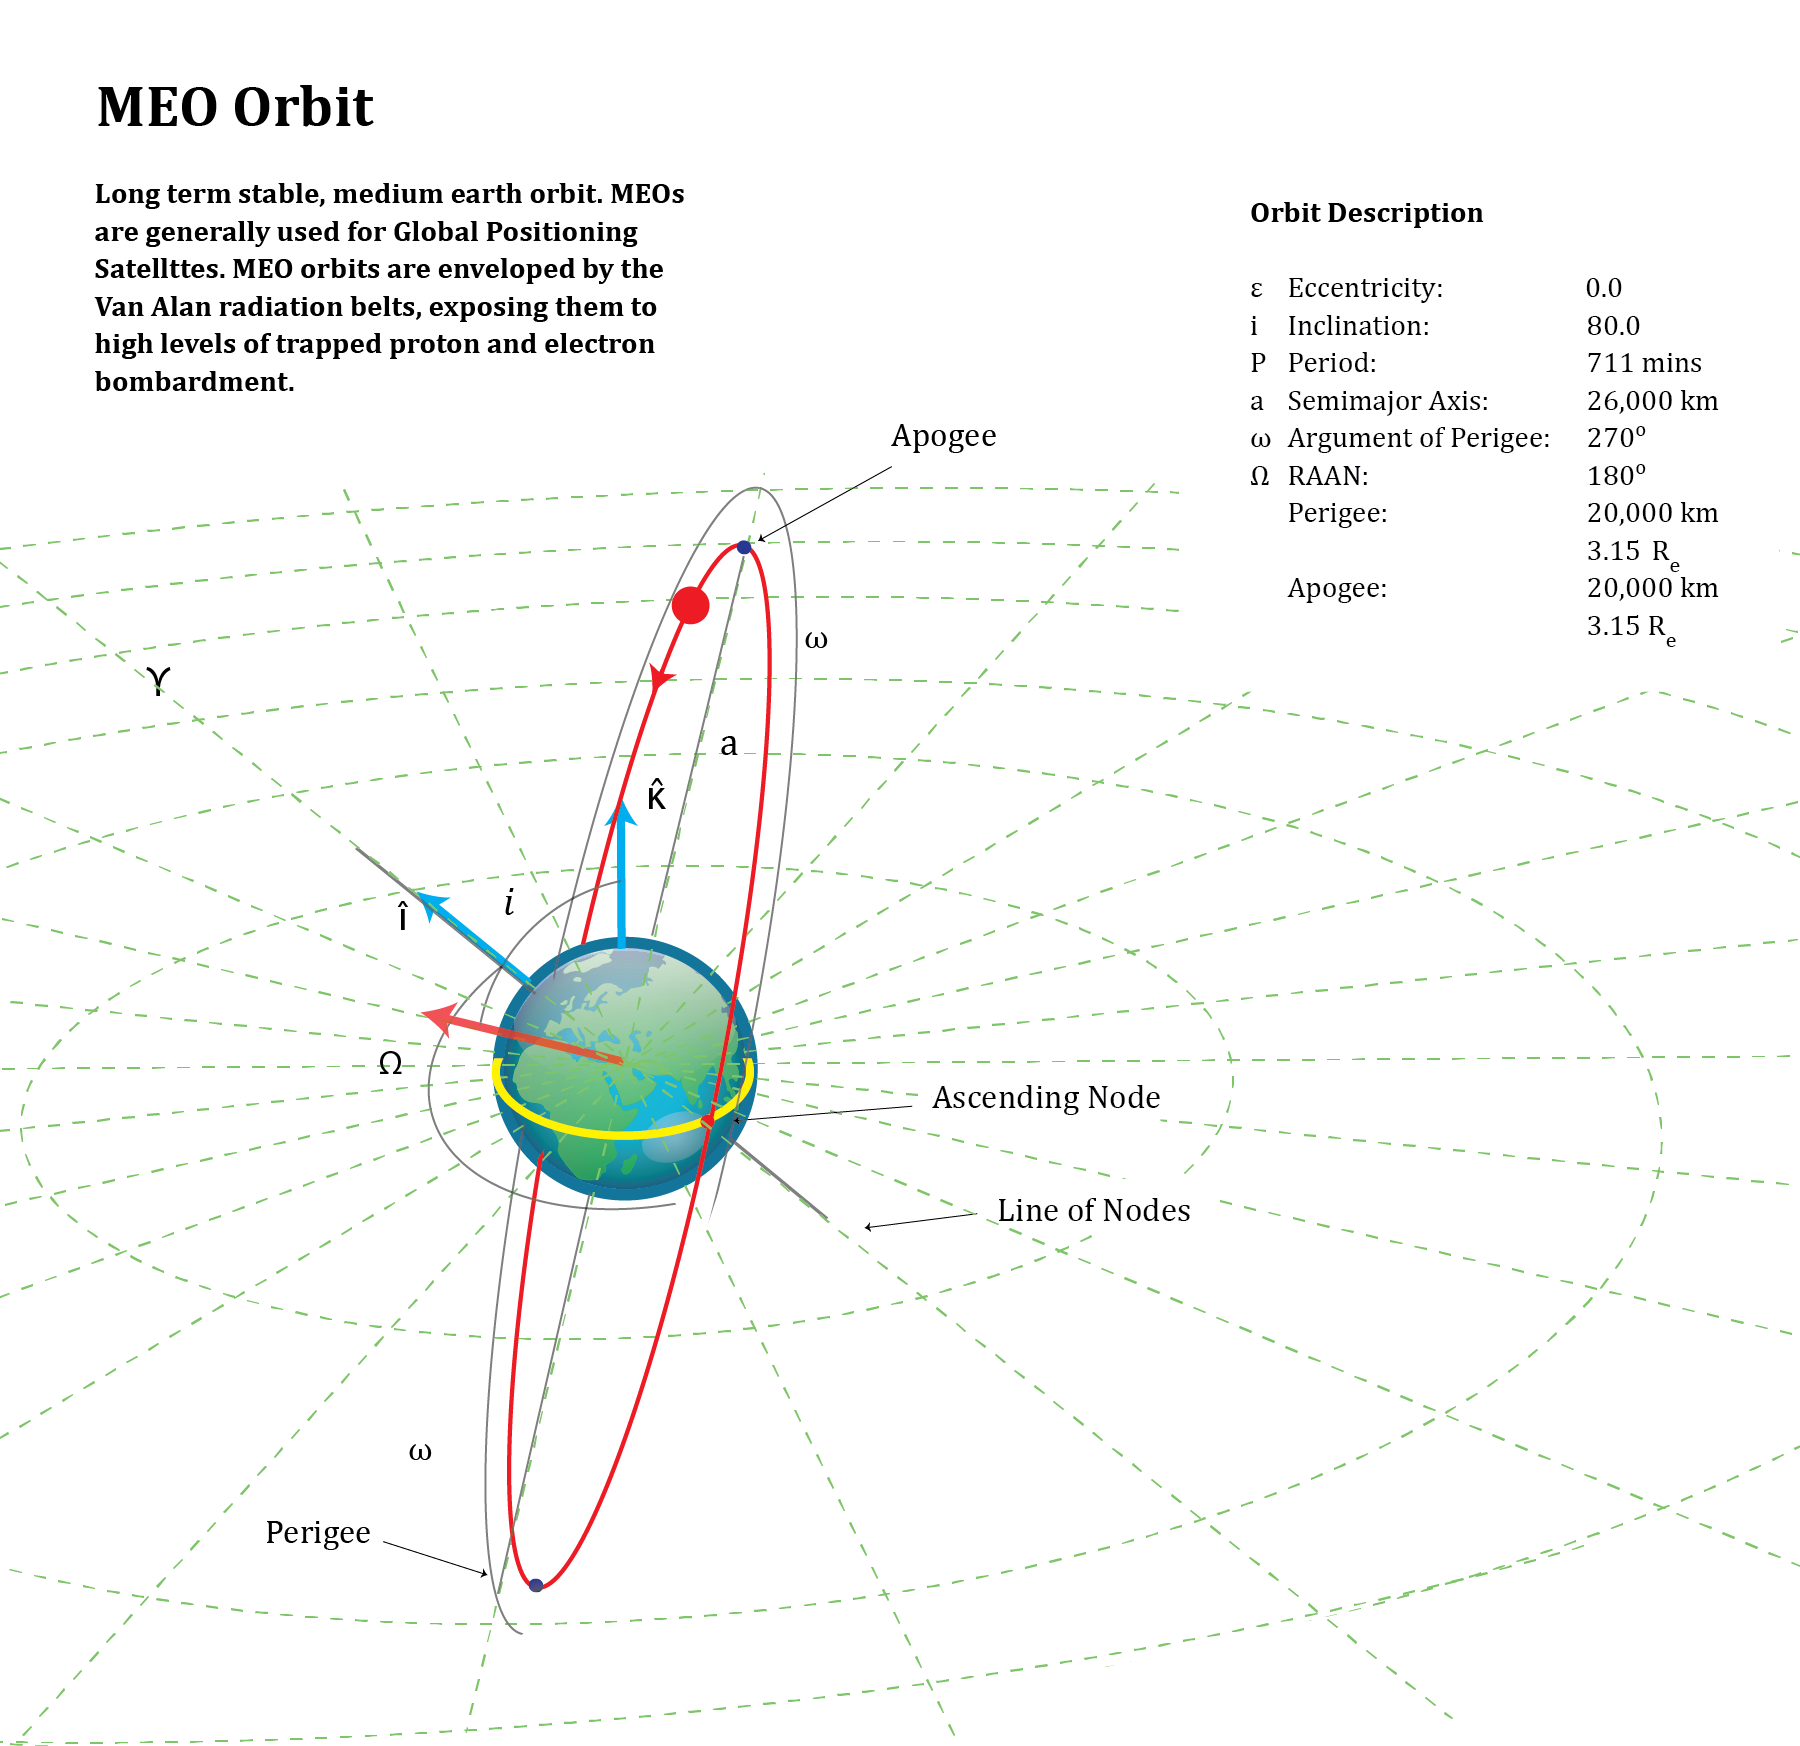
\includegraphics[height=5in]{OHB_MEO_Orbit.png}
    \caption{The Medium Earth Orbit and description.}
    \label{fig:OHBMEO}
\end{figure}

\section{Orbits}

Four different orbits are presented in the following sections. Three are geocentric. one heliocentric. One of the geocentric orbits, the Medium Earth Orbit (MEO), was provided by a potential contractor. Another, the Molniya orbit, is a common Highly Elliptical Orbit (HEO) type that is frequently considered for astronomical imaging missions. The third, the P/2 HEO. is an orbit utilized by the Transiting Exoplanet Survey Satellite (TESS) mission, a mission similar to Pearl. The heliocentric orbit, called the Earth Trailing Orbit (ETO), is one that was first used by the Spitzer Space Telescope.

\subsection{MEO-Type Orbits}

A potential contractor has strongly recommended one of two Medium Earth Orbit trajectories; either a MEO with a 70 to 80 degree inclination, or an Equatorial MEO (EMEO).

\begin{figure}[!b]
    \centering
    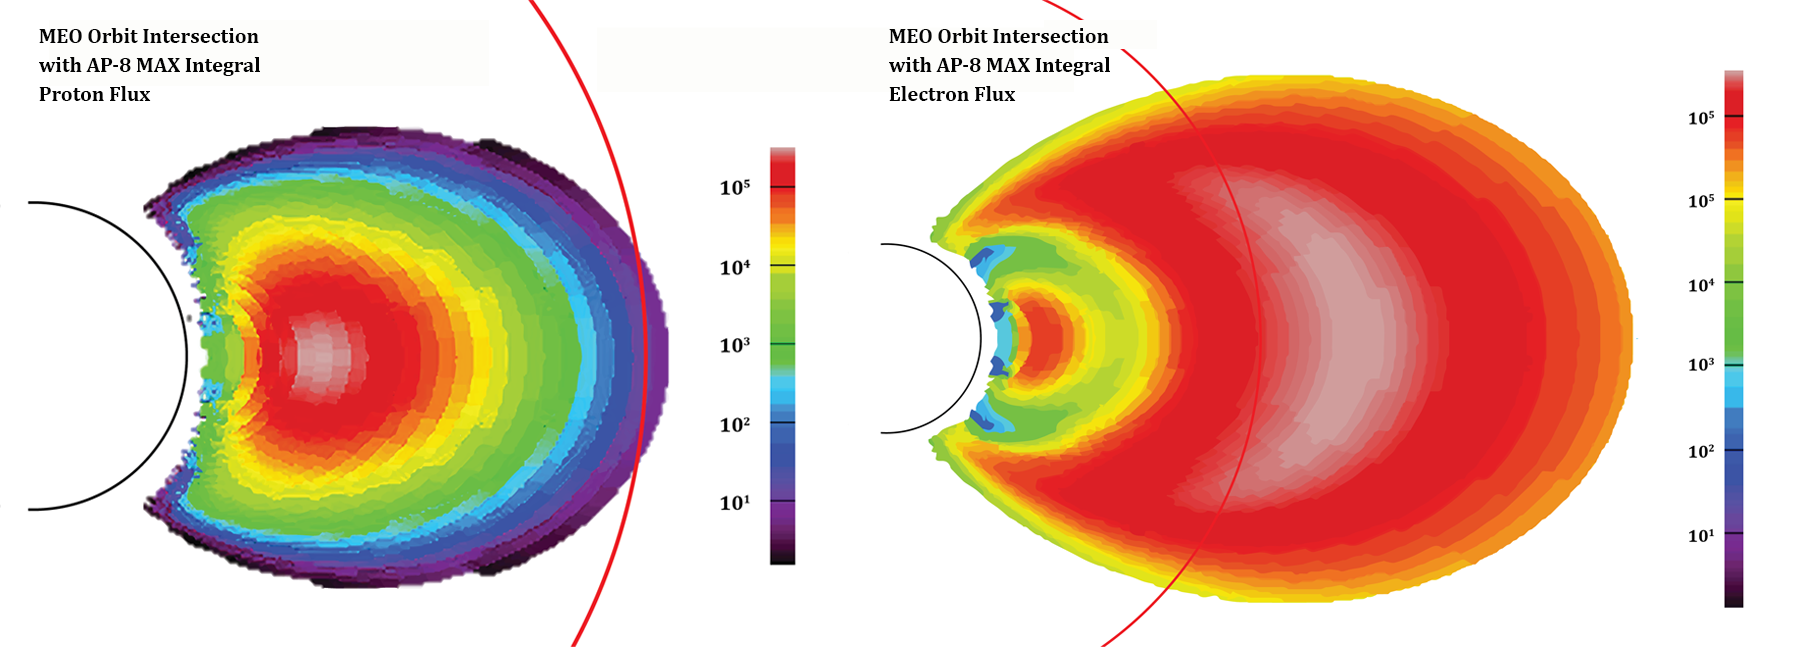
\includegraphics[height=2in]{MEO_Flux.png}
    \caption{The MEO Orbital Intersection with the Van Allen proton and electron regions. Scale units are MeV per centimeter squared per second.}
    \label{fig:OHBMEOVAB}
\end{figure}

\subsubsection{The Medium Earth Orbit}

Figure~\ref{fig:OHBMEO} is a diagram of the MEO orbit at a 70\degree~inclination and with contractor specified orbital parameters. It is fully circular ($\epsilon=0$) with both apogee and perigee at 3.15 Earth radii. MEO orbits are typically used for global positioning and communications satellites, and complete roughly two orbits in a 24 hour period. They are highly unusual orbits to be considered for astronomical imaging missions for a number of reasons, including exposure to thermal effects from Earth's heat radiation, solar radiation pressure trajectory perturbations, and insufficient integration times due to the short orbital period. High energy trapped particles are problematic in this orbit as well. Figure~\ref{fig:OHBMEOVAB} shows a plot of the intersection of the orbit with the high energy proton and electron regions of the Van Allen Belts (VAB).

\subsubsection{The Equatorial Medium Earth Orbit}

The EMEO trajectory is also circular, lies in the plane of the Earth's equator, and Is fully embedded in both the Proton and Electron zones of the VAB: this is shown in Figure~\ref{fig:OHBEMEOVAB}. Although in the lower energetic portion of the Proton region, continuous 24 hour exposure to a 10 MeV proton flux sums to a large total fluence over the lifetime of the mission. 

The high energy electron situation is far worse: the satellite would be continuously exposed to a $10^5$ MeV electron flux over the lifetime of the mission. Exposure to high energy electrons is now being looked at as the cause of 26 hard failures in eight satellites over a period of sixteen years. Satellites in these orbits are heavily shielded and use radiation hardened equipment to protect against the extreme high energy proton and electron environment.

\begin{figure}[!t]
    \centering
    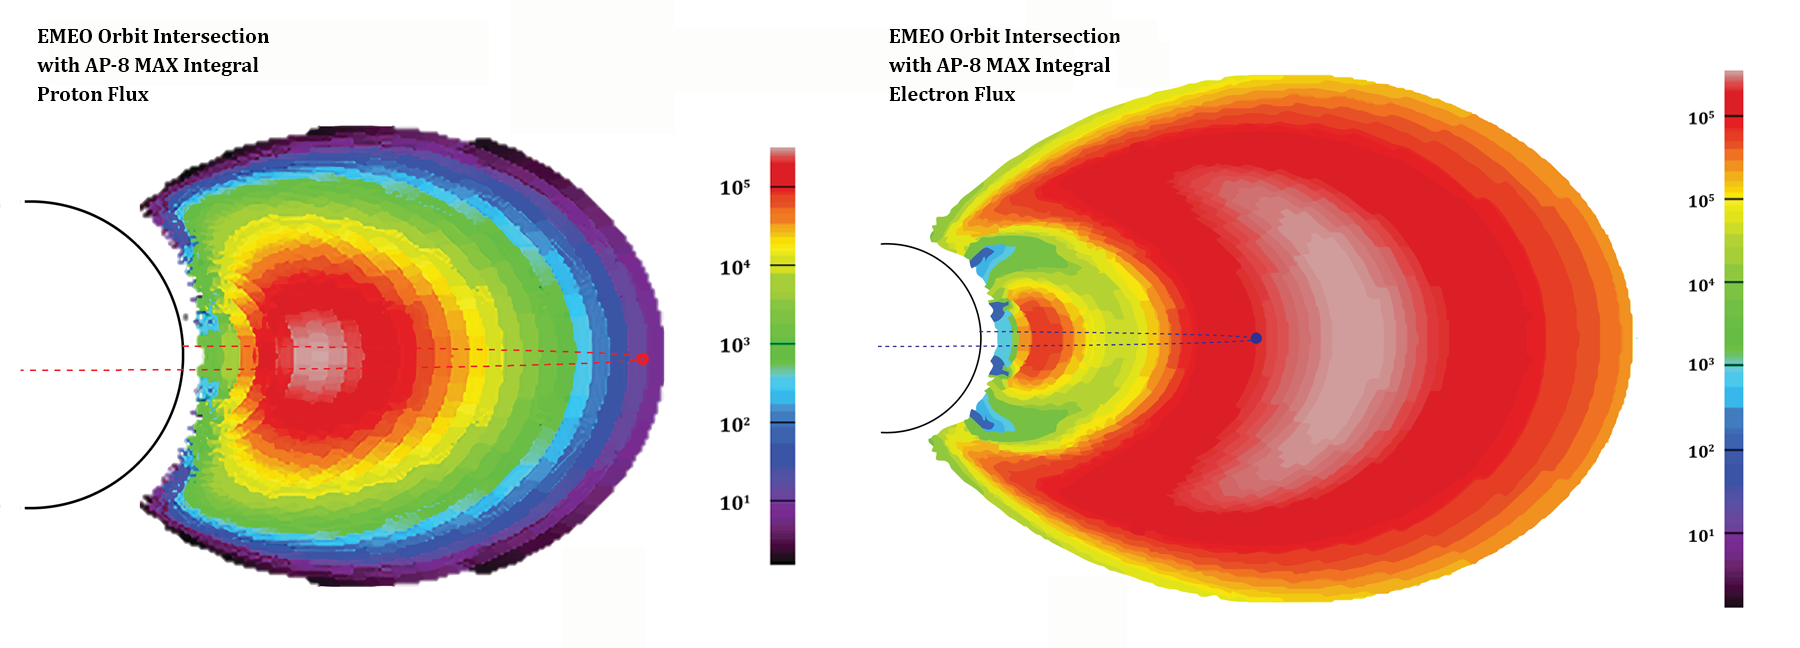
\includegraphics[height=2in]{EMEO_Flux.png}
    \caption{The EMEO Orbital Intersection with the Van Allen proton and electron regions. Scale units are MeV per centimeter squared per second.}
    \label{fig:OHBEMEOVAB}
\end{figure}

\subsection{Molniya Orbit}

The Molniya orbit is named after the Russian word for lightning for its rapid passage through perigee. The orbit was originally designed for communications satellites and has a large dwell time at apogee over its hemisphere of interest. It has a relatively low $\Delta V$ to orbit, but has sizable station-keeping requirements. 

\begin{figure}[H]
    \centering
    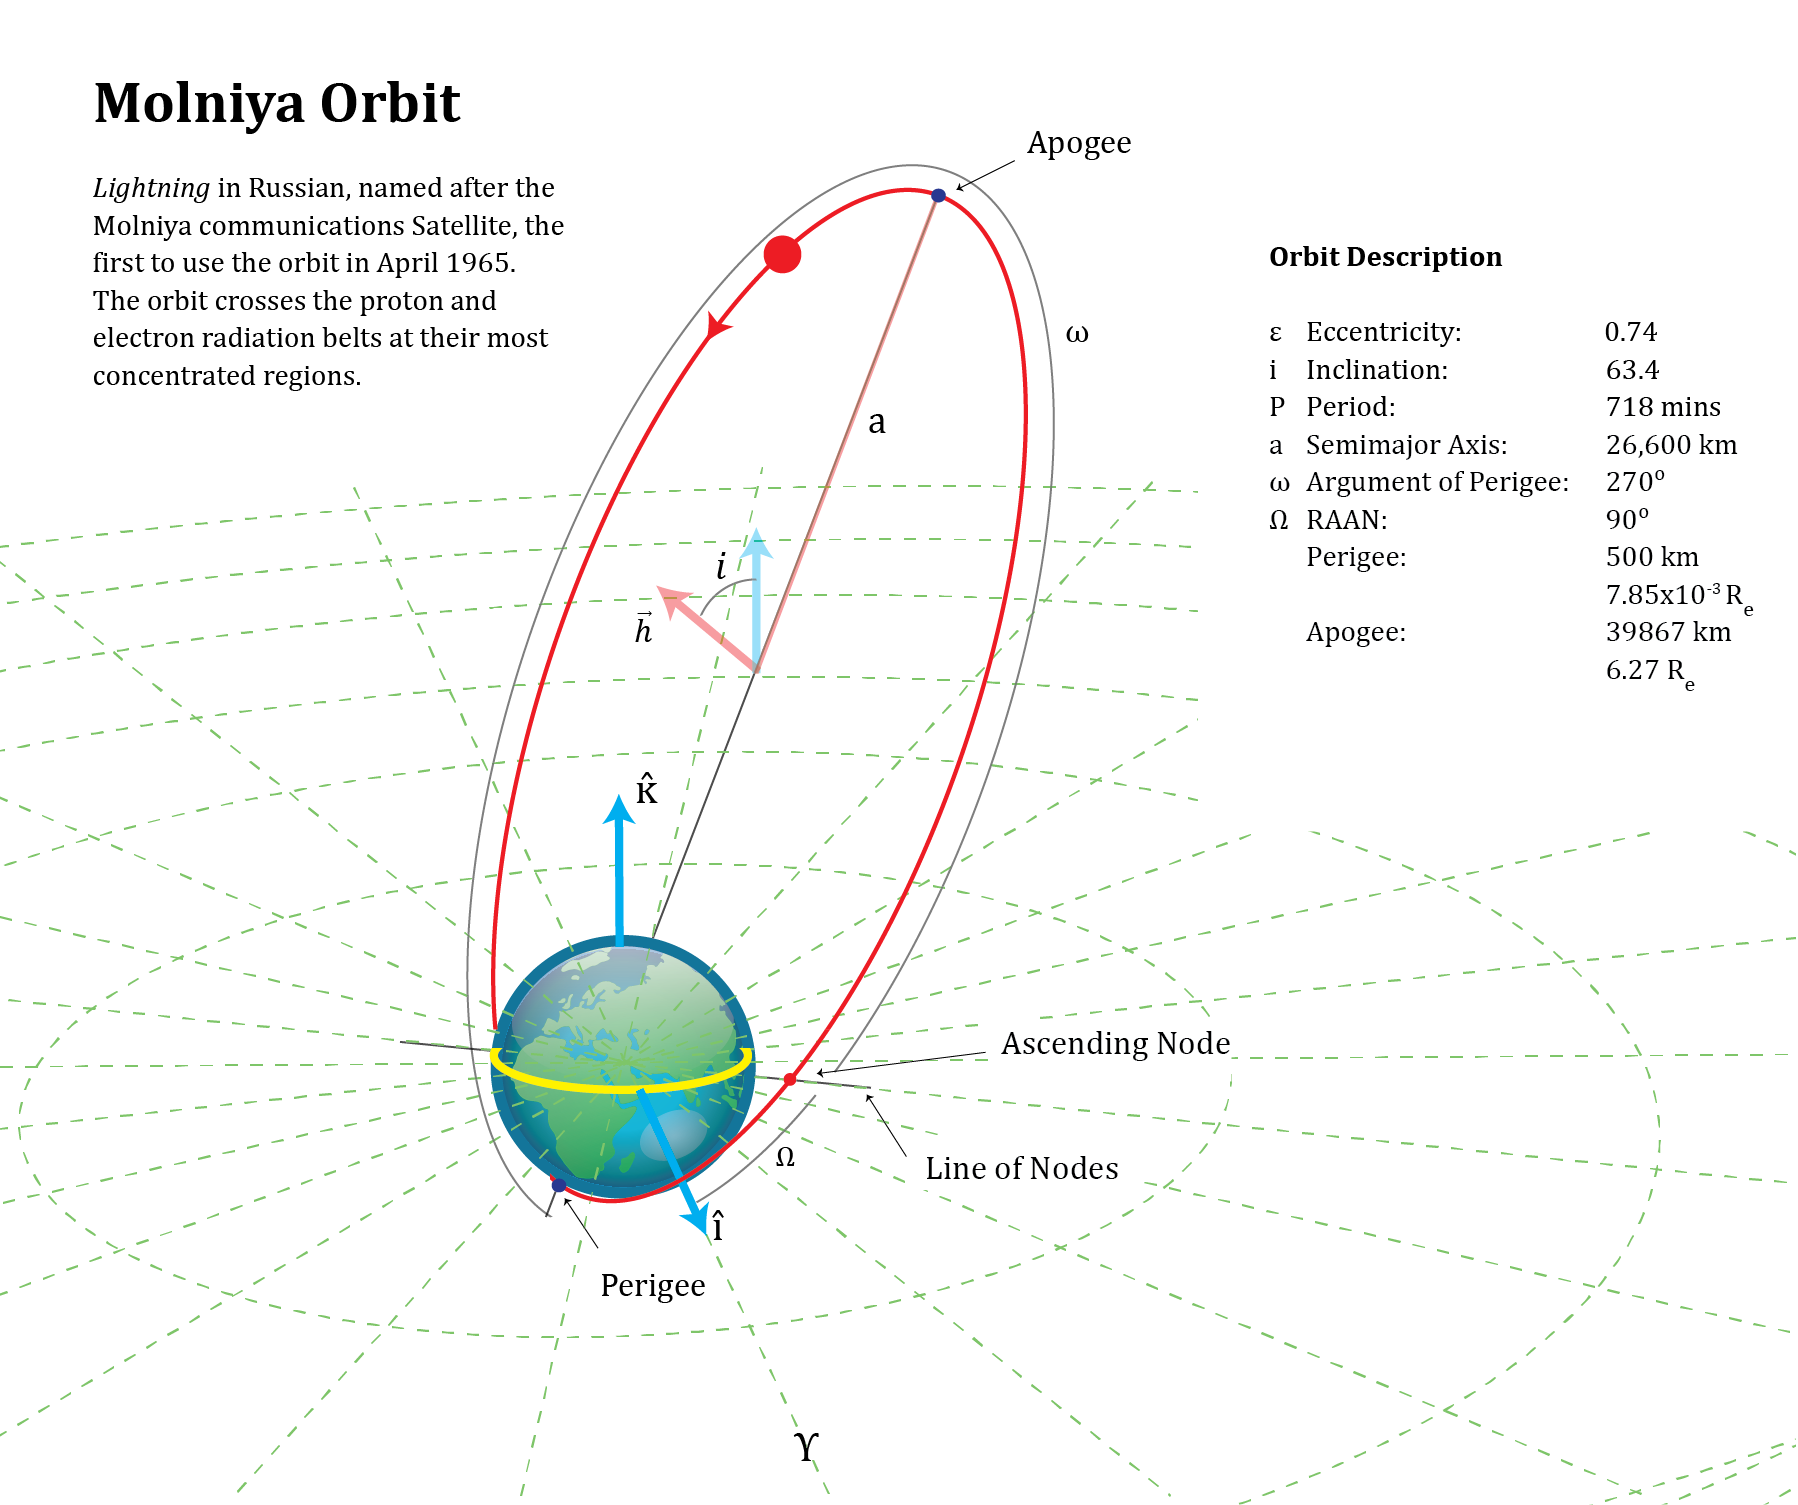
\includegraphics[height=4.55in]{assets/Molniya_Diagram.png}
    \caption{The Molniya orbit and orbit description.}
    \label{fig:MOL_Orbit}
\end{figure}

\begin{figure}[H]
    \centering
    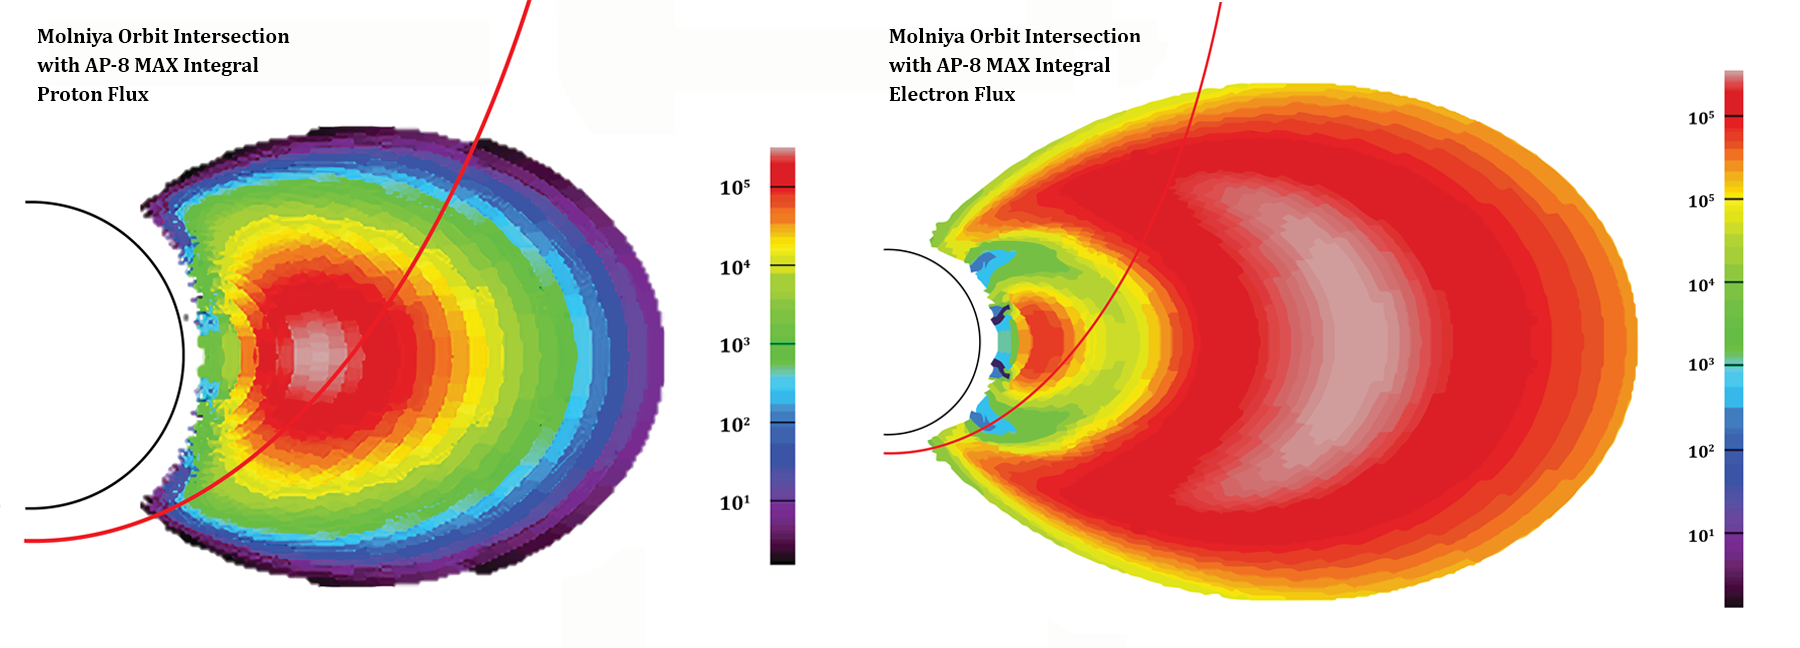
\includegraphics[height=2in]{assets/Molniya_Flux.png}
    \caption{The Molniya Orbital Intersection with the Van Allen proton and electron regions. Scale units are MeV per centimeter squared per second.}
    \label{fig:MOLVAB}
\end{figure}

Its rapid passage through perigee also makes communications with the satellite difficult, as a ground station must have steerable antennas to track the spacecraft, and rapid range changes cause variations in signal amplitude. The orbit also requires the satellite to pass through the VABs four times per day. The orbit is illustrated in Figure~\ref{fig:MOL_Orbit}, and its intersection with the Van Allen proton and electron regions is shown in Figure~\ref{fig:MOLVAB}. 

\begin{figure}[H]
    \centering
    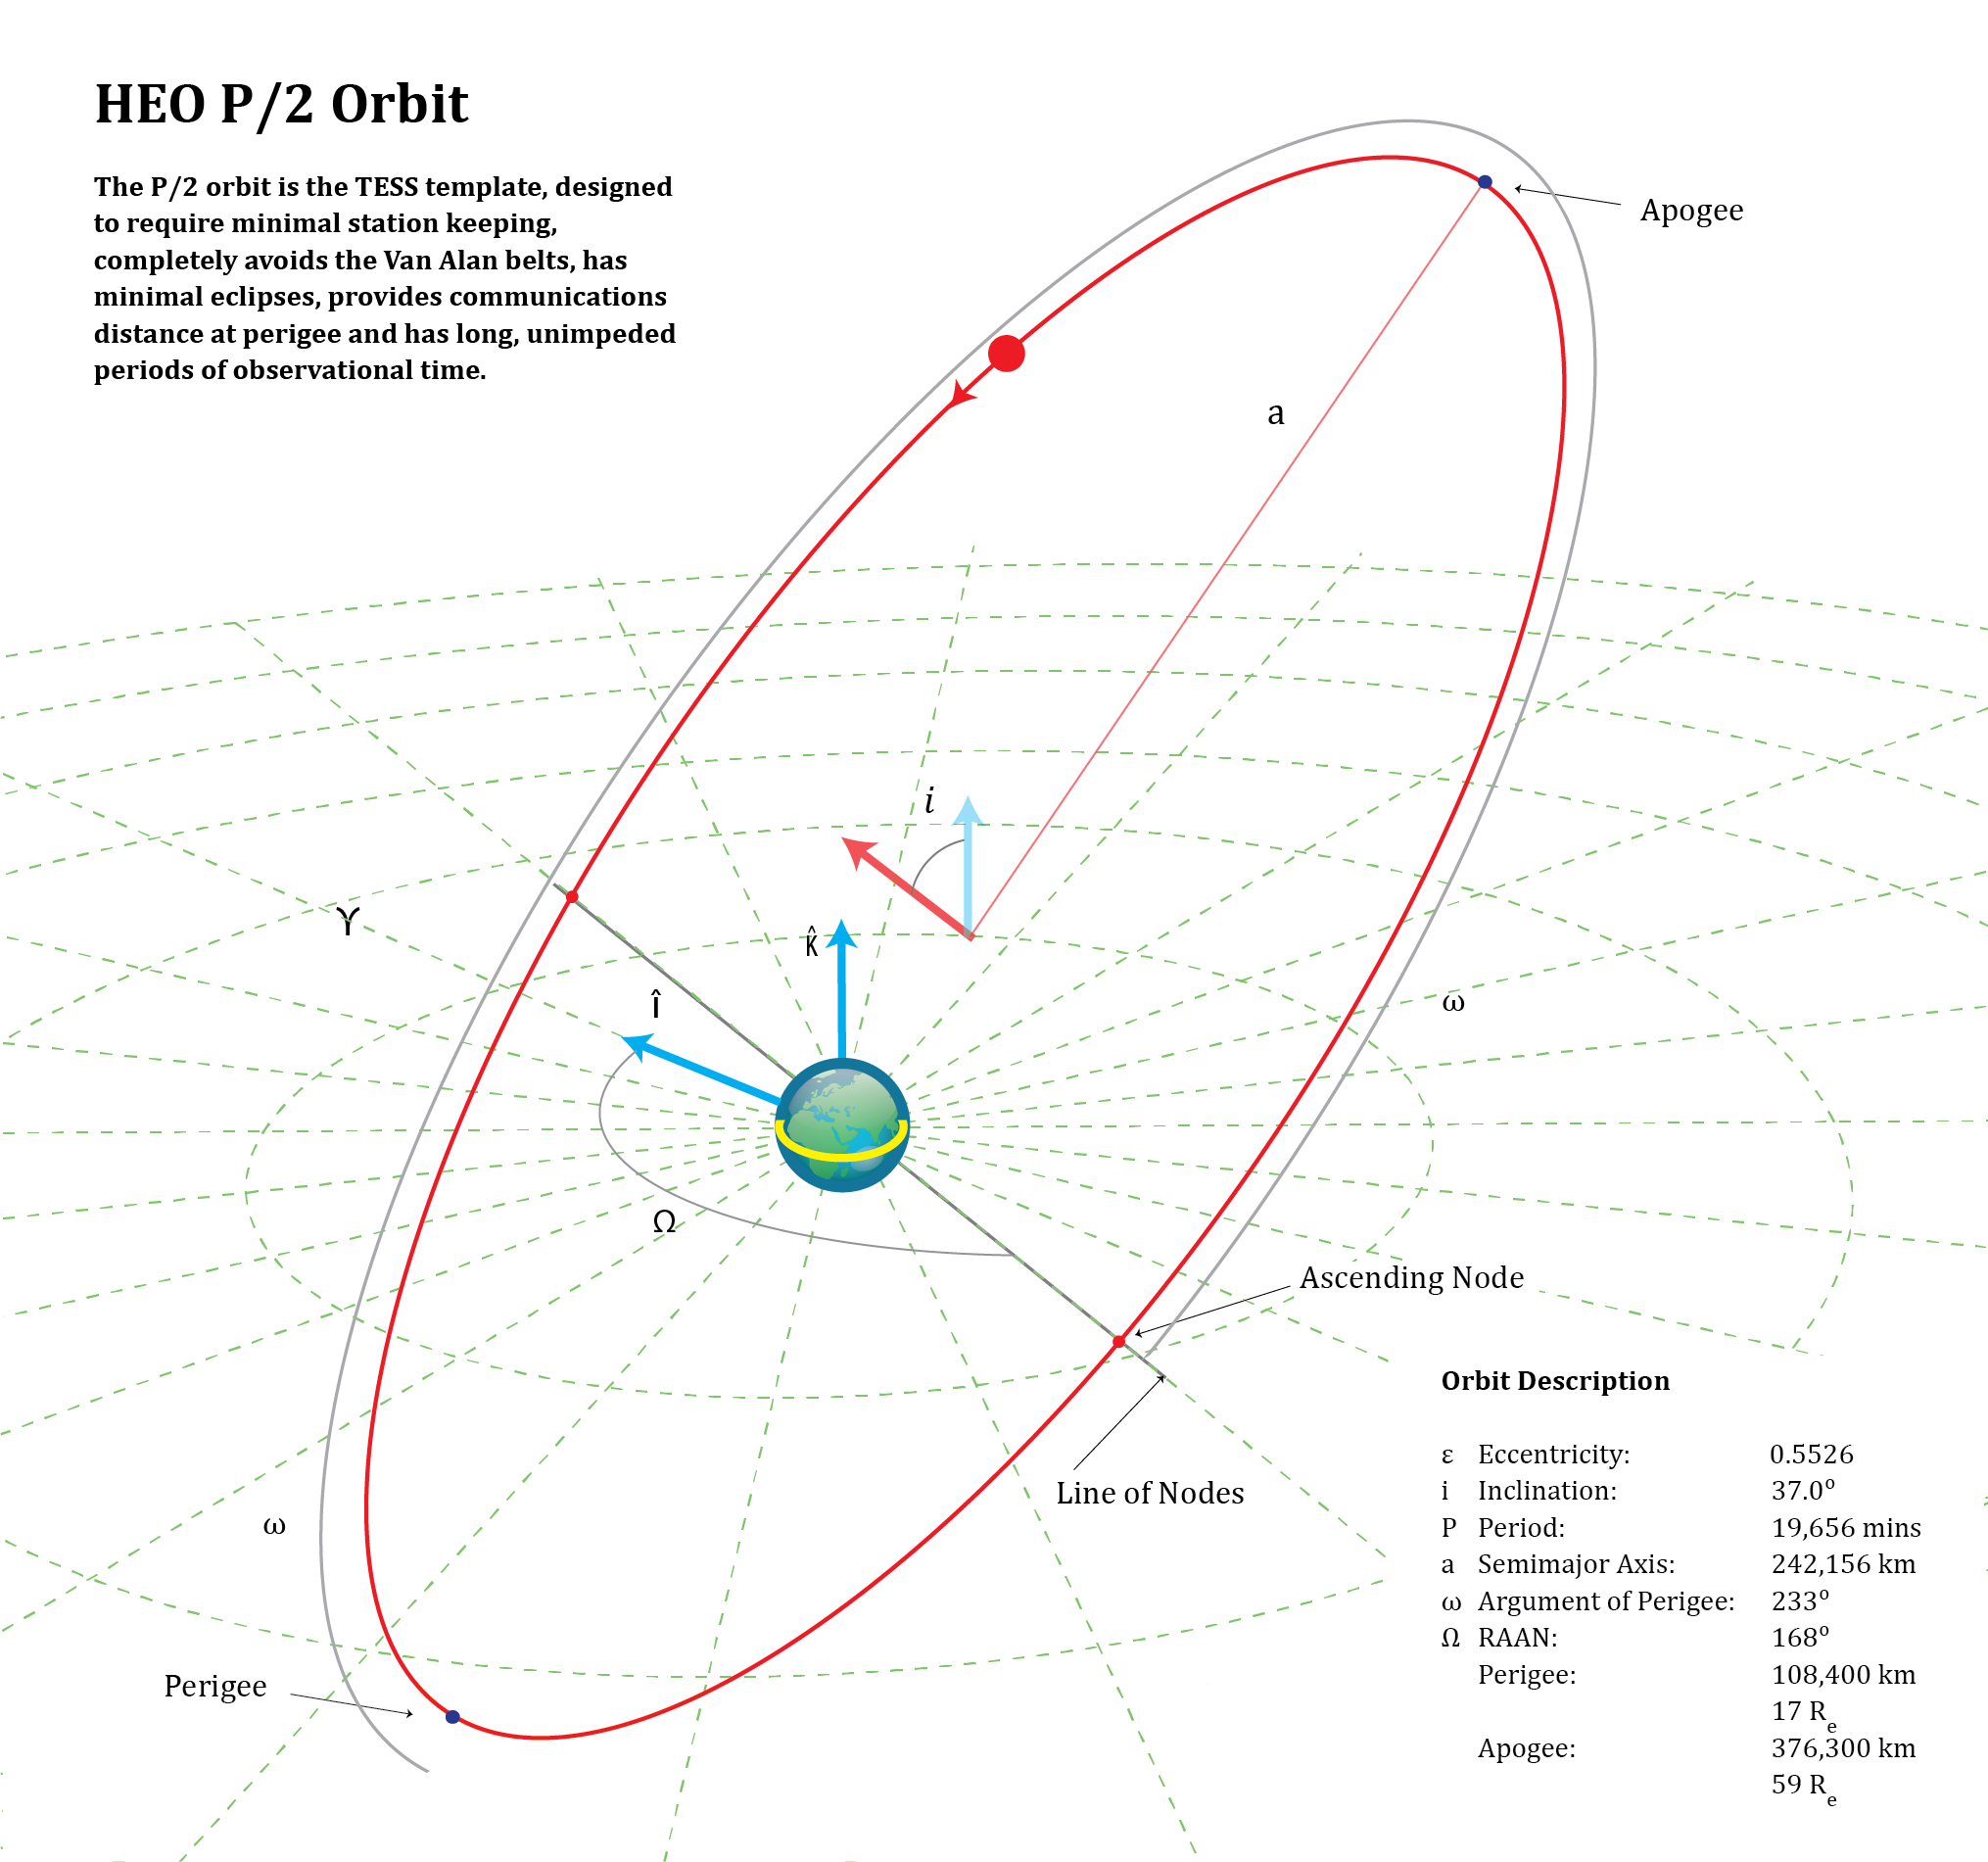
\includegraphics[height=4.8in]{TESS_Diagram.png}
    \caption{The P/2 HEO TESS Orbit diagram and description.}
    \label{fig:TESS_Orbit}
\end{figure}

\begin{figure}[H]
    \centering
    \begin{minipage}{\dimexpr.5\textwidth-1em}
        \centering
        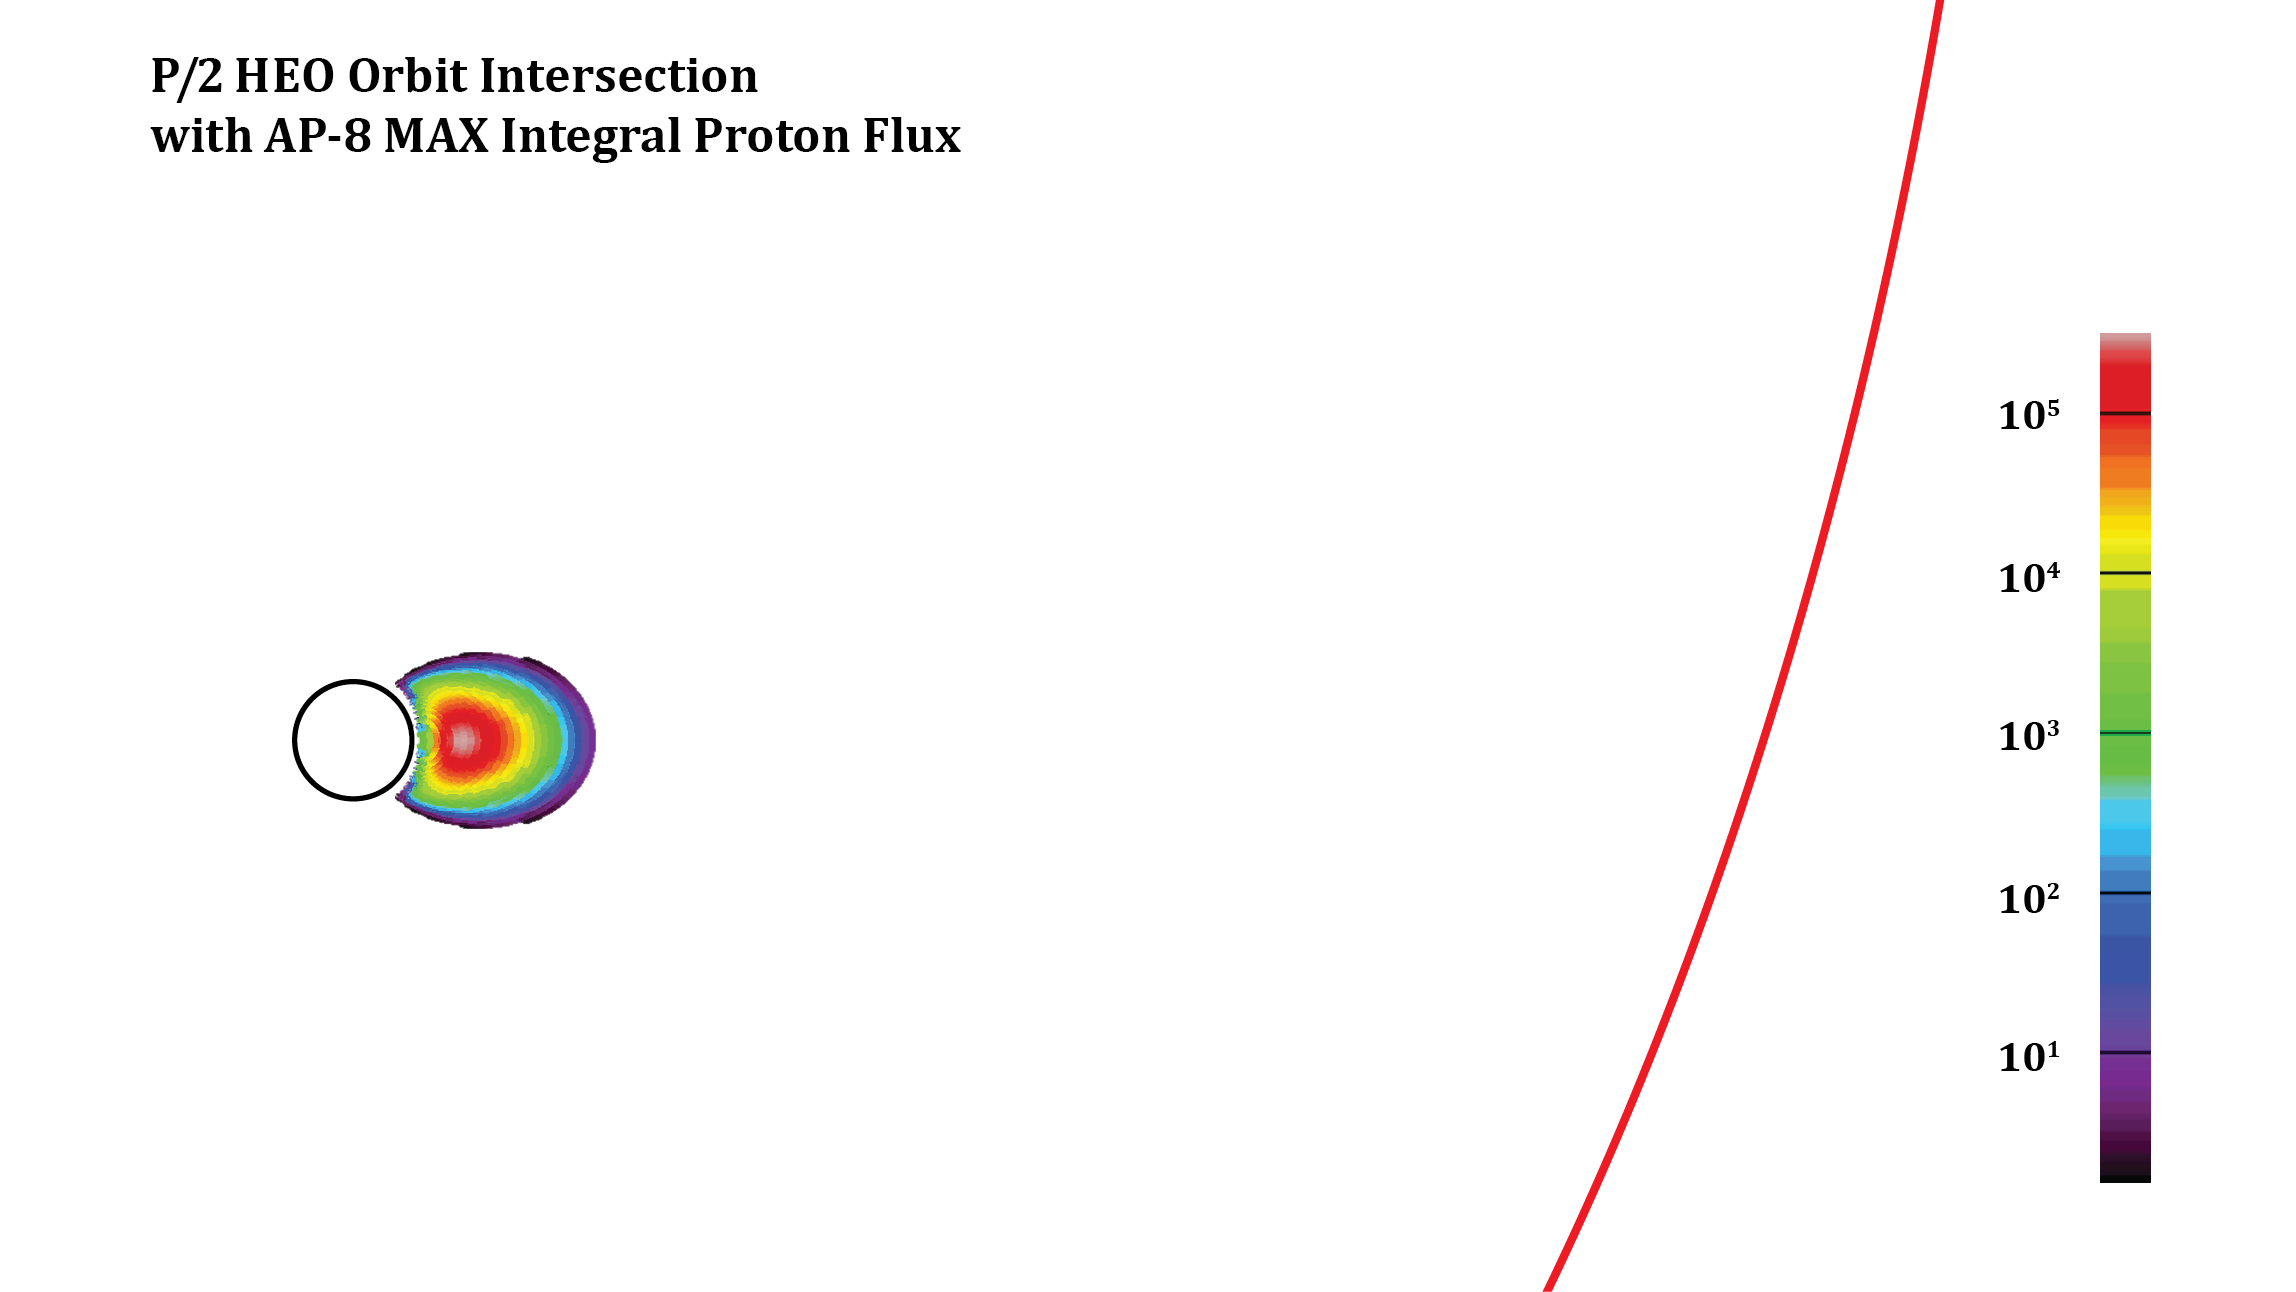
\includegraphics[width=1\linewidth]{TESS_PFlux.png}
        \caption{The P/2 HEO TESS Orbital Intersection, or lack thereof, with the Van Allen proton regions.}
        \label{fig:TESS_Pflux}
    \end{minipage}\hfill
    \begin{minipage}{\dimexpr.5\textwidth-1em}
        \centering
        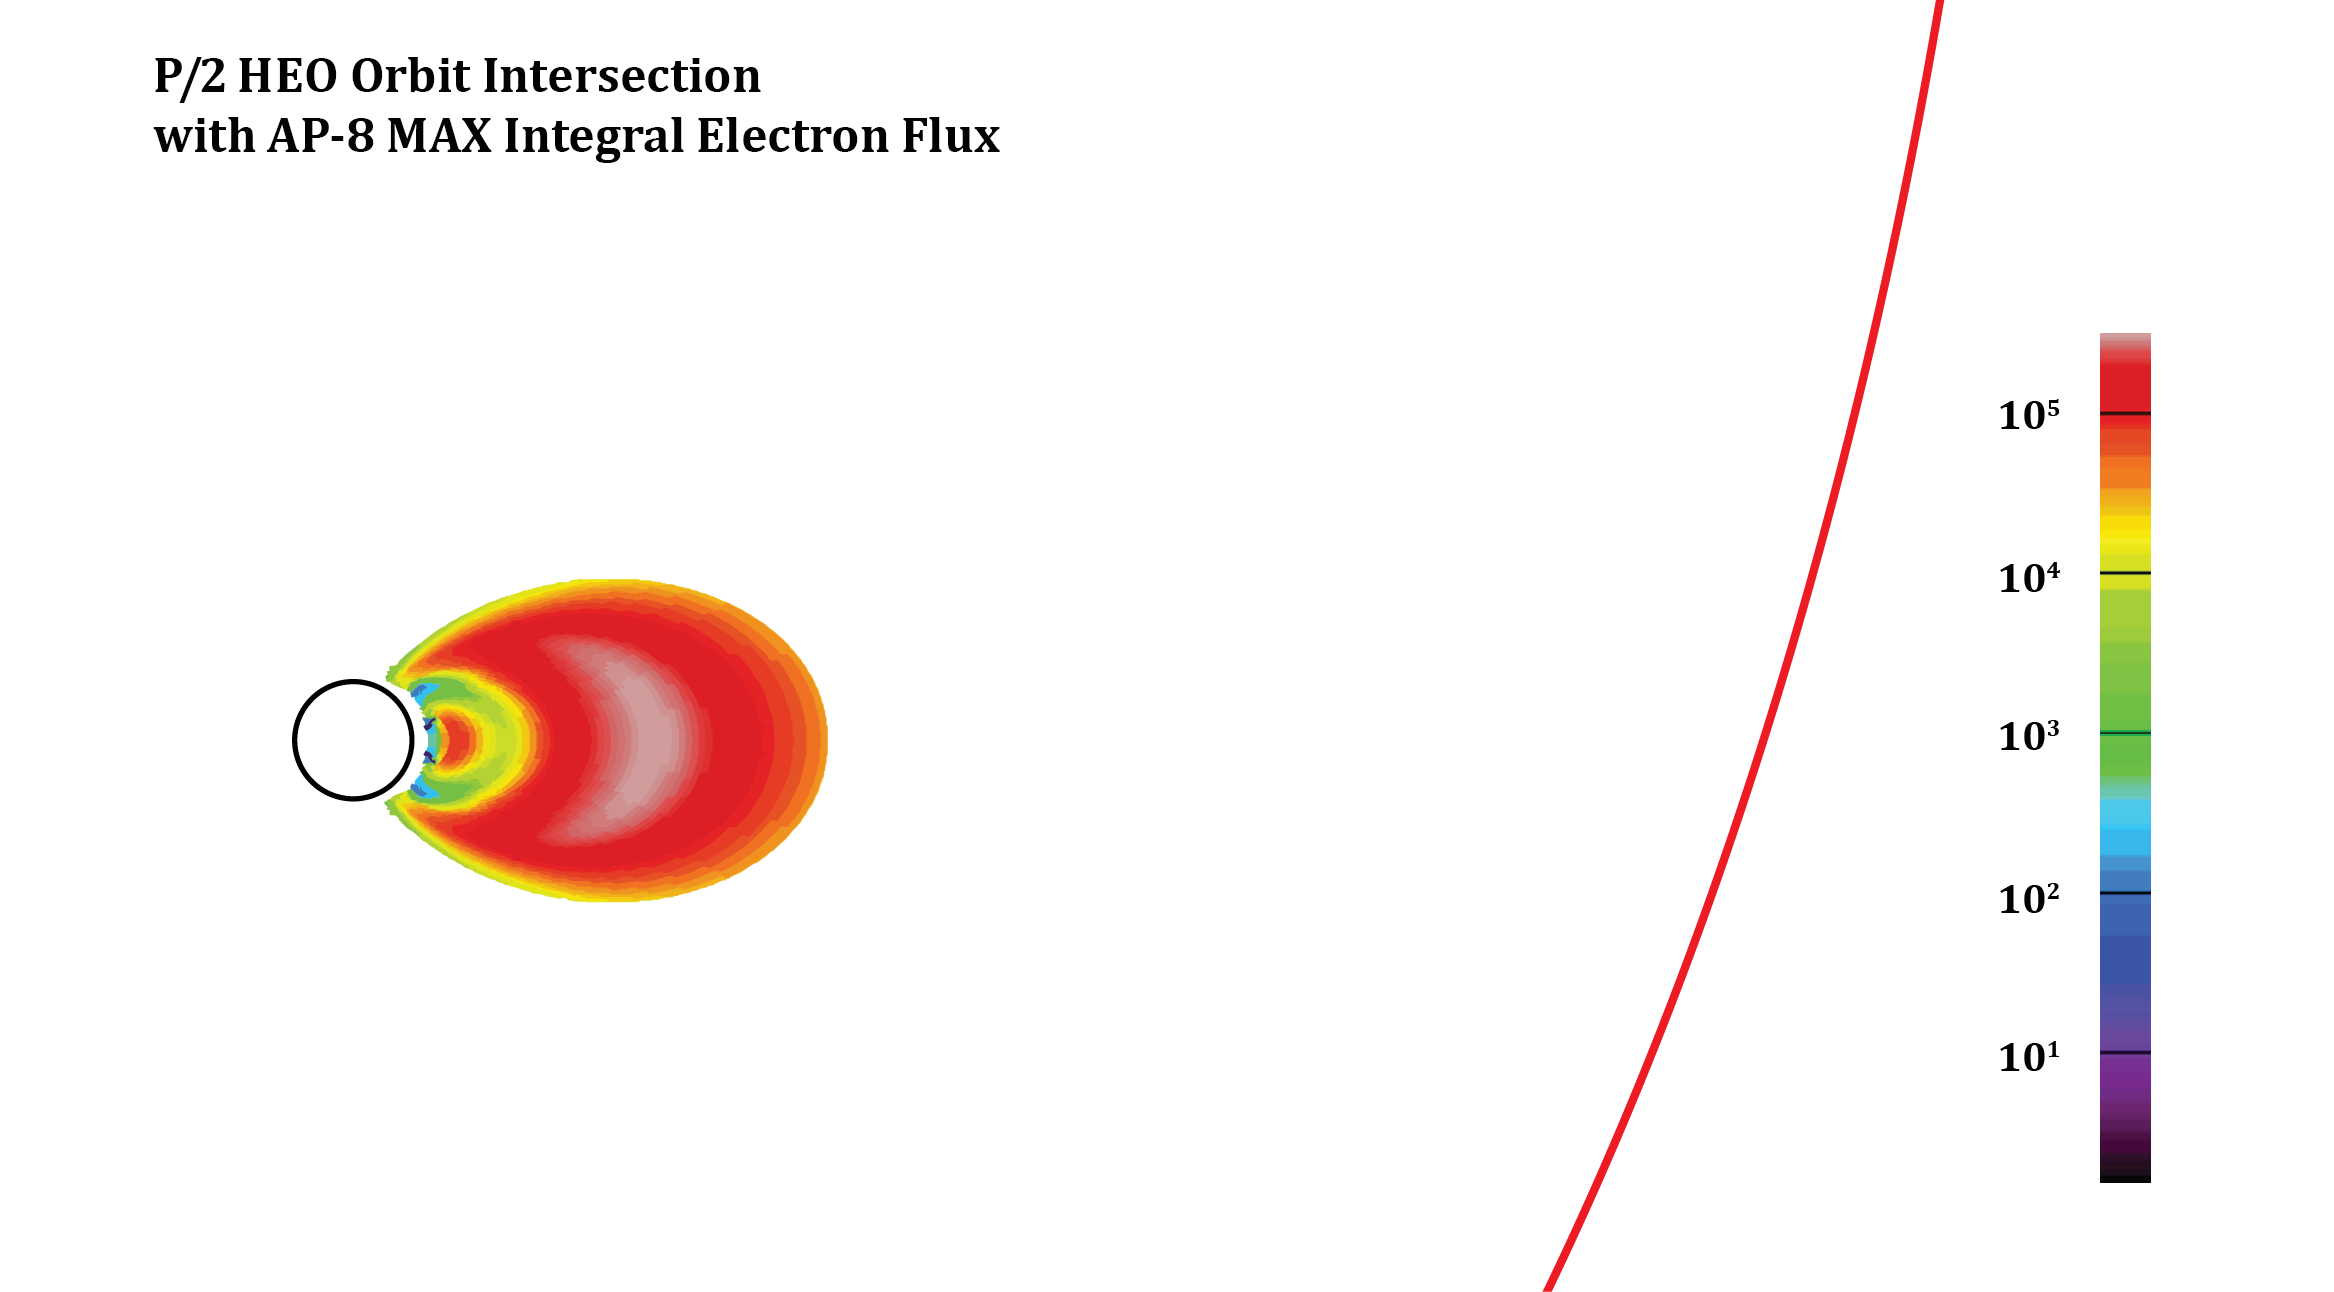
\includegraphics[width=1\linewidth]{TESS_EFlux.png}
        \caption{The P/2 HEO TESS Orbital Intersection, or lack thereof, with the Van Allen electron regions.}
        \label{fig:TESS_Eflux}
    \end{minipage}
\end{figure}

\subsection{P/2-HEO Orbit (TESS)}
The P/s HEO orbit is well suited for exoplanet imaging missions. It has been used for this type of mission before: The Transiting Exoplanet Survey Satellite, or TESS.

The P/2-HEO orbit is a highly elliptical, high earth orbit in 2:1 resonance with the moon, shown in Figure~\ref{fig:TESS_Orbit}. First studied by McGiffin and Mathews in 2001, it was eventually utilized for the Transiting Exoplanet Survey Satellite mission. Its perigee lies above GEO altitude,  its apogee is beyond the moon's orbital radius, and it completely avoids the Van Allen Belts (Figures~\ref{fig:TESS_Eflux} and \ref{fig:TESS_Pflux}). Through clever design, it balances solar and lunar perturbations, creating a highly stable orbit with a lifetime of decades while virtually eliminating the need for station keeping. 

Its perigee altitude is ideal for communications, and its apogee provides long, unobstructed views that easily accommodate long imaging integration times. It also has a large trade space of possible designs to accommodate mission requirements. These designs all require relatively modest $\Delta V$, between 175 \unit{m/s} and 400 \unit{m/s}, depending on the specific orbit and launch site.\cite{mcgiffin01} For more detail on the TESS orbit, see the internal memo 'The Argument for the P/2 HEO Orbit'.

\subsection{Earth-Trailing Orbit}

\subsubsection{Description}

Essentially, the Earth Trailing Orbit (ETO) \textit{is} the Earth's orbit, but with a smaller eccentricity ($\epsilon_{ETO}=0.011$ vs $\epsilon_{Earth}=0.0167$), a longer period ($P_{ETO}=372.2$ days vs $P_{Earth}=365.2$ days), and an inclination of $1.13\degree$ to the plane of the Earth's orbit. The satellite trails the earth, and recedes at approximately 0.12 AU per year. The orbit diagram is shown in Figure~\ref{fig:ETO_Orbit}.

The Spitzer infrared space telescope and the Kepler Planet-Finder space telescope both used the ETO. The benefits of the ETO orbit include avoiding the gravitational and torque effects of earth orbit and avoiding Earth occultations. 

\paragraph{Advantages of the ETO Orbit}

\begin{itemize}[noitemsep]
 \item Absence of Eclipses;
 \item Stable Thermal Configuration;
 \item High Observing Efficiency;
 \item No need for station keeping.
\end{itemize}

\begin{figure}[H]
    \centering
    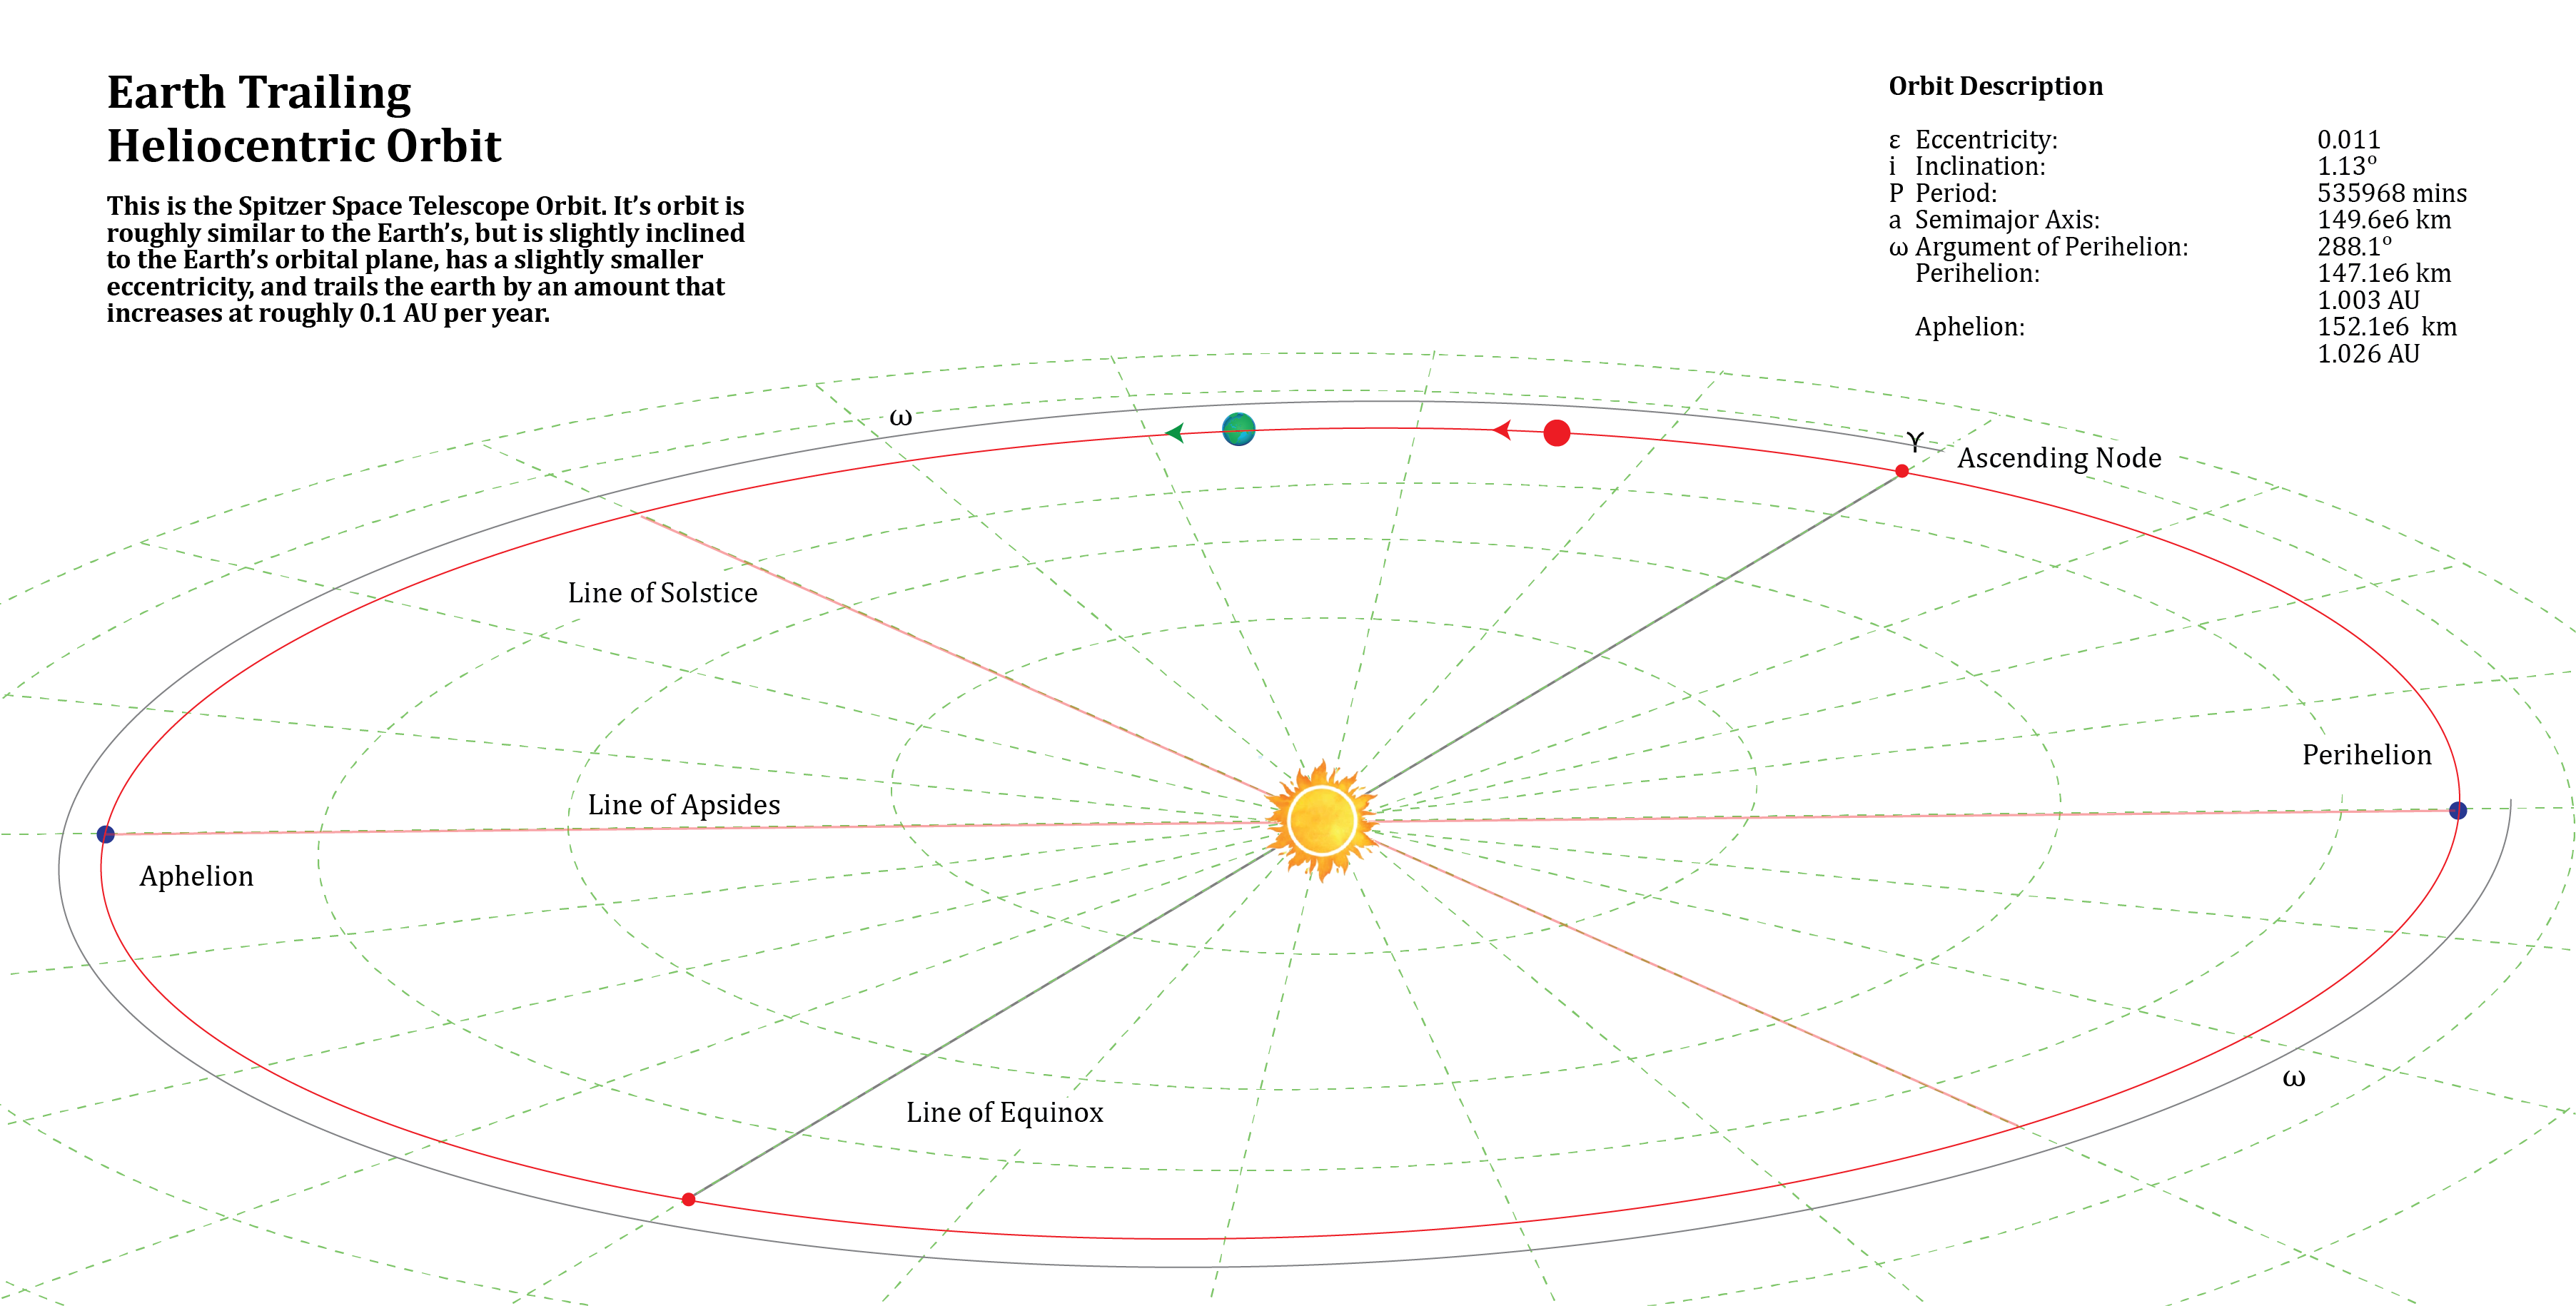
\includegraphics[height=3.0in]{ETO_Diagram.png}
    \caption{The Earth Trailing Orbit and description.}
    \label{fig:ETO_Orbit}
\end{figure}
\paragraph{Disadvantages of the ETO Orbit}

\begin{itemize}[noitemsep]
 \item Power requirement for communication increases as satellite recedes;
  \item Launch to orbit $\Delta V$ is in excess of 4,000 m/s~\cite{joffre18};
 \item Orbit is outside of the Magnetosphere, leading to:
 \begin{itemize}[noitemsep]
            \setlength{\itemindent}{-.2in}
                 \item Greater susceptibility to solar proton storms;
                 \item Higher quiescent galactic cosmic flux rate.
            \end{itemize}       
\end{itemize}

\section{Orbit Radiation}

\subsection{A few Notes}

\subsubsection{Note on ETO Radiation Data}
\label{sec:ETORadData}

The Earth-Trailing Orbit (ETO) cannot easily be modeled with SPENVIS; in order to do so, the heliocentric  parameters would need to be expressed in geocentric terms, producing epicycles and deferents that would make Ptolemy cringe. Therefore, data from the National Oceanic and Atmospheric Administration's (NOAA) Geostationary Operational Environmental Satellites, R Series (GEOS-R), can be used to provide insight into the nature of the ETO Solar Energetic Particle (SEP) environment.

Previous generation GEOS satellites carry a Space Environment Monitor (SEM) instrumentation package which includes an Energetic Particle Sensor (EPS) instrument. The EPS onboard GEOS-13 through GEOS-15 measures protons from 80 keV to 100s of MeV. In addition, GEOS-4 through GEOS-15 included a High Energy Proton and Alpha Detector (HEPAD) instrument which measures high energy proton fluxes above ~350 MeV in four broadband channels.\cite{kress21} The current generation of GEOS satellites, starting with GEOS-16, have replaced the original SEM package with the new five instrument Space environment In-Situ Suite (SEISS) package. Two of these instruments are the Solar and Galactic Proton Sensor (SGPS) units, facing in opposite directions. SPGS measures protons with energies from 1 to >500 MeV in fourteen channels. Solar Proton Events (SPEs) occurring in July and September of 2017 enables cross calibration between the EPS and SGPS instruments.\cite{kress21}

In the 2022 Astronomy \& Astrophysics article 'Annual Integral Solar Proton Fluences' \cite{Raukunen22}, the authors use data from GEOS Satellites to provide solar proton fluences from 1984 to 2019. These fluences show the expected variability resulting from the 11-year solar cycle, and are thus extremely useful for evaluating the ETO's potential SEP exposure.

\subsubsection{Notes on Simulations}
\label{sec:notes}
All Trapped Proton Fluxes and Fluences simulations and all Solar Particle Fluences simulations were run with the same parameters. No simulations took into account spaceship shielding to simplify the simulation setup.

\paragraph{Trapped Proton Fluxes and Fluences}
These simulations examine the Van Allen Belt proton flux along the spacecraft's trajectory, and were run using the standard AP8/AE8 model set at solar maxima. The internal magnetic field model is GSFC 12/66 120, update 1970.\cite{website:spenvis01} Trajectory parameters are as shown on the orbit illustrations, for a one year mission duration with science orbit commencing 00:00:00 01 January 2025.

\paragraph{Solar Particle Fluences}
Solar particle modeling was conducted with SPENVIS Emission of Solar Protons (ESP), for total fluence using worst case events.\cite{website:spenvis02} All available ions, from Hydrogen to Uranium, were selected. Magnetosphere shielding was set as Eccentric Dipole/Quiet Magnetosphere/Unchanged Magnetic Moment/All Arrival Directions. Confidence level that fluences would not be exceded was set to 95\%. Trajectory parameters are as shown on the orbit illustrations, for a one year mission duration with science orbit starting 00:00:00 January 1st 2025.

\begin{figure}[H]
    \centering
    \begin{minipage}{\dimexpr.5\textwidth-1em}
        \centering
        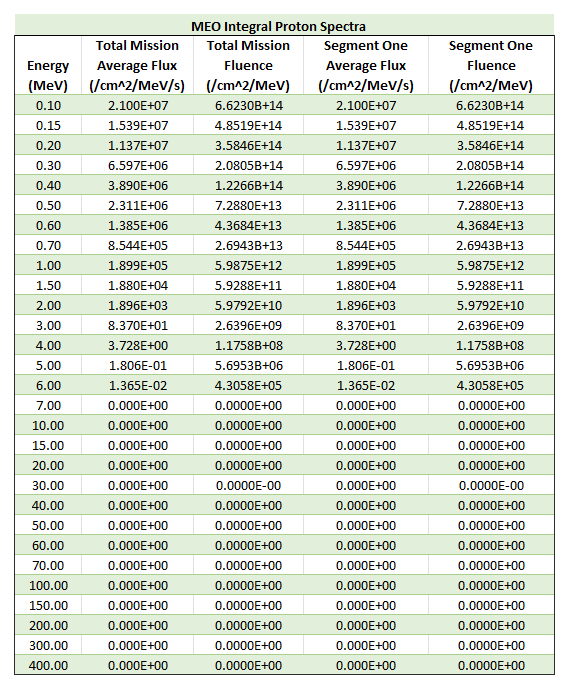
\includegraphics[width=1\linewidth]{MEO_TPSM_PS.png}
        \caption{The MEO Solar Maxima trapped proton fluxes and fluences, Integral Spectra.}
        \label{fig:OHBMEOIPS}
    \end{minipage}\hfill
    \begin{minipage}{\dimexpr.5\textwidth-1em}
        \centering
        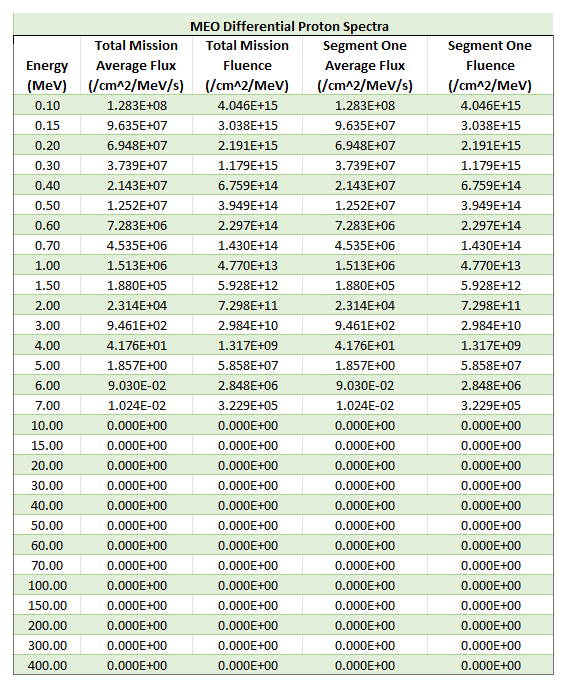
\includegraphics[width=1\linewidth]{MEO_TPSM_DPS.png}
        \caption{The MEO Solar Maxima trapped proton fluxes and fluences, Differential Spectra.}
        \label{fig:OHBMEODPS}
    \end{minipage}
\end{figure}

% --------------------------------------------------
\subsection{MEO Orbit Simulations}

\subsubsection{Trapped Proton Fluxes and Fluences}

I have only shown results for the MEO orbit, as the high energy electron exposure for the EMEO orbit immediately disqualifies it from  consideration. Figure~\ref{fig:OHBMEOIPS} above shows the MEO Orbit AP8 SPENVIS Integral Proton Spectra output; Figure~\ref{fig:OHBMEODPS} above shows the AP8 SPENVIS Differential Proton Spectra output.

\subsubsection{Solar Particle Fluences}
The MEO Orbit solar particle spectrum is shown in Figure~\ref{fig:OHBMEOSP}.

% --------------------------------------------------

\subsection{Molniya Orbit Simulations}

\subsubsection{Trapped Proton Fluxes and Fluences}

 Figure~\ref{fig:MolniyaIPS} below shows the Molniya orbit AP8 SPENVIS Integral Proton Spectra output; Figure~\ref{fig:MolniyaDPS} below shows the AP8 SPENVIS Differential Proton Spectra output.

\subsubsection{Solar Particle Fluences}

The Molniya Orbit solar particle spectrum is shown in Figure~\ref{fig:MolniyaSP}.

\begin{figure}[!b]
    \centering
    \begin{minipage}{\dimexpr.5\textwidth-1em}
        \centering
        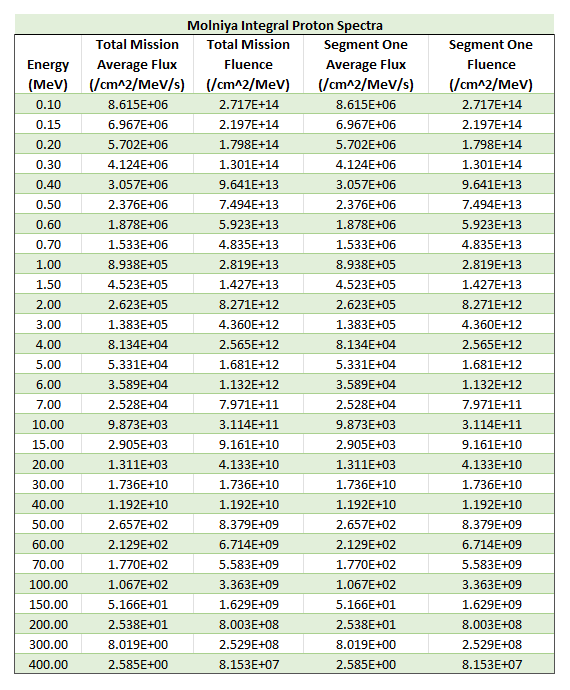
\includegraphics[width=1\linewidth]{Molinya_IPS.png}
        \caption{The Molniya Solar Maxima trapped proton fluxes and fluences, Integral Spectra.}
        \label{fig:MolniyaIPS}
    \end{minipage}\hfill
    \begin{minipage}{\dimexpr.5\textwidth-1em}
        \centering
        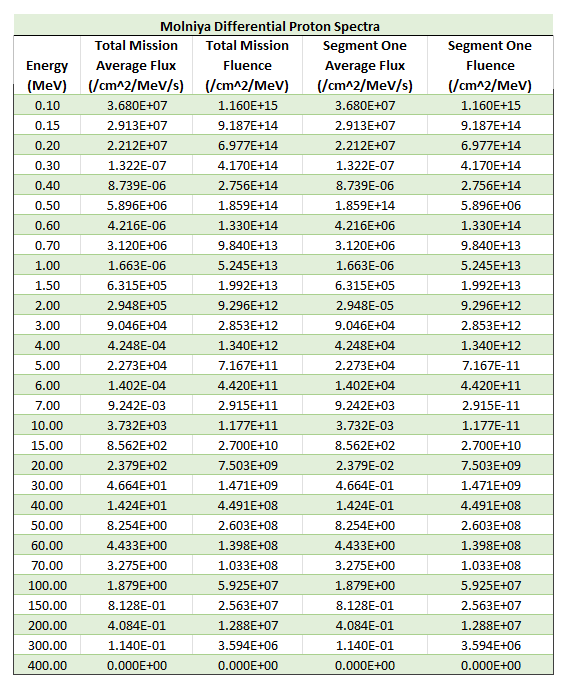
\includegraphics[width=1\linewidth]{Molinya_DPS.png}
        \caption{The Molniya Solar Maxima trapped proton fluxes and fluences, Differential Spectra.}
        \label{fig:MolniyaDPS}
    \end{minipage}
\end{figure}

\begin{figure}[H]
    \centering
    \begin{minipage}{\dimexpr.5\textwidth-1em}
        \centering
        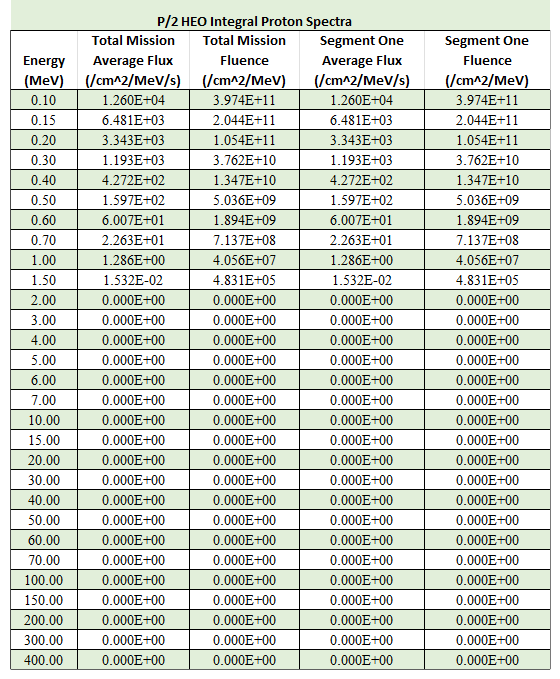
\includegraphics[width=1\linewidth]{HEO_IPS.png}
        \caption{The P/2 HEO (TESS) Solar Maxima trapped proton fluxes and fluences, Integral Spectra.}
        \label{fig:P2HEOIPS}
    \end{minipage}\hfill
    \begin{minipage}{\dimexpr.5\textwidth-1em}
        \centering
        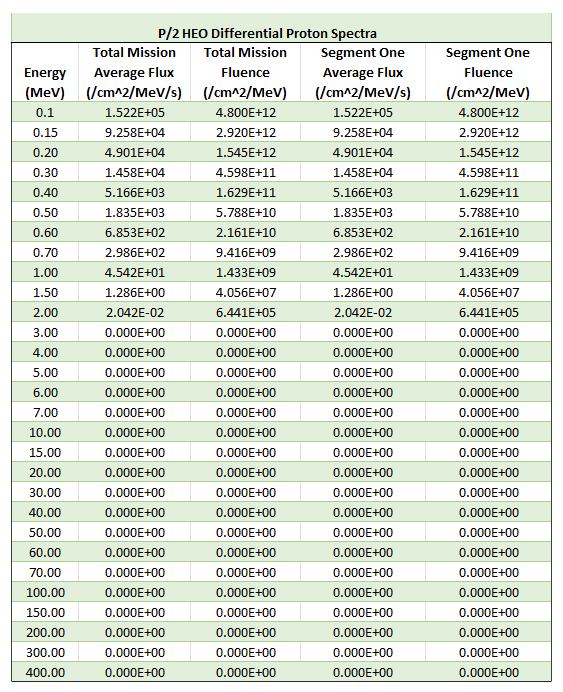
\includegraphics[width=1\linewidth]{HEO_DPS.png}
        \caption{The P/2 HEO (TESS) Solar Maxima trapped proton fluxes and fluences, Differential Spectra.}
        \label{fig:P2HEODPS}
    \end{minipage}
\end{figure}

\subsection{P/2 HEO TESS Orbit Simulations}

\subsubsection{Trapped Proton Fluxes and Fluences}

Figure~\ref{fig:P2HEOIPS} above shows the P/2 HEO Orbit AP8 SPENVIS Integral Proton Spectra output; Figure~\ref{fig:P2HEODPS} above shows the AP8 SPENVIS Differential Proton Spectra output.

\subsubsection{Solar Particle Fluences}

The P/2 HEO TESS solar particle spectrum is shown in Figure~\ref{fig:TESSSP}.

\subsection{Earth Trailing Orbit Data}
\label{sec:GEOS}

As the ETO is, by definition, outside the region of the Van Allen Belts, the only relevant radiation data concerns high energy solar particles. The following data is from the National Oceanic and Atmospheric Administration's (NOAA) Geostationary Operational Environmental Satellites, R Series (GEOS-R), as discussed in Section~\ref{sec:ETORadData}.

The chart shown in Figure~\ref{fig:ETORad} below shows annual integral solar fluences for the years 1984 - 2019, along with error values, in units of particles per \unit{$cm^{-2}$}. Each column in the chart alternates between a fluence bin that \textit{begins} at the given energy level indicated by the subscript, and an error value for that bin. On the right side of the chart is an ordering of the $F_{10 MeV}$ fluences by year (the green bars are meaningless here). The years 1989, 2000, 2001 and 2003 were the most active recent years in terms of solar particle events. A chart of solar proton events for the years 1976 through 2017 is presented in the appendix.

\begin{figure}
    \centering
    \begin{minipage}{\dimexpr.5\textwidth-1em}
        \centering
        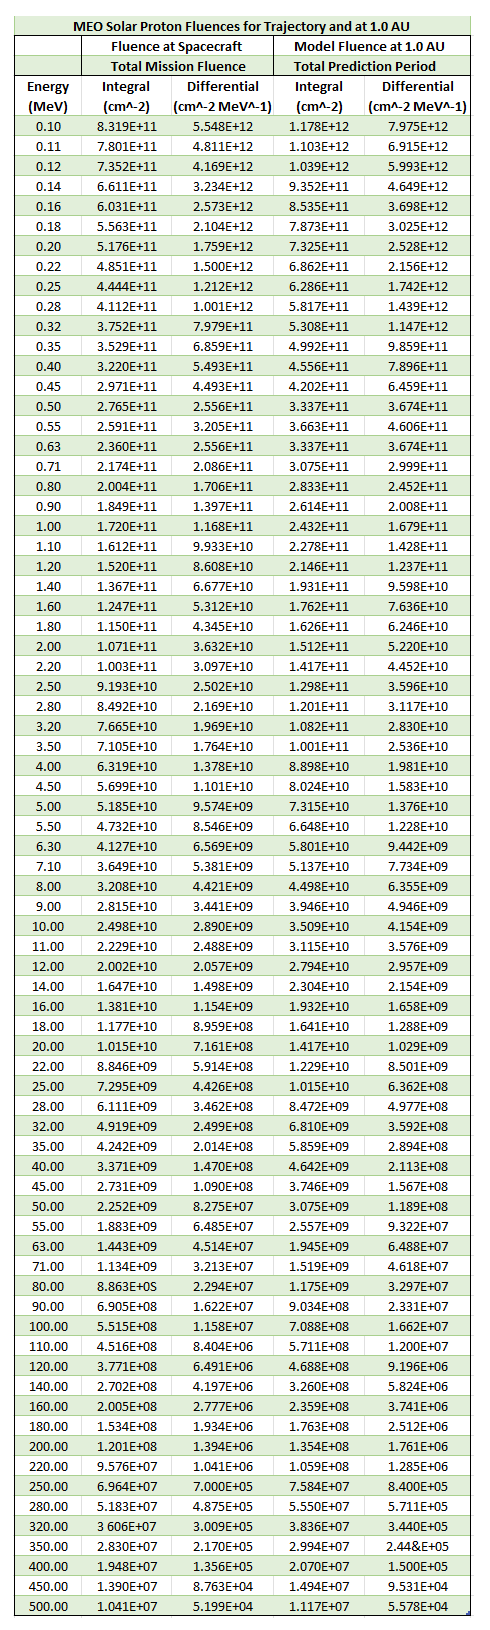
\includegraphics[width=0.78\linewidth]{MEO_SP.png}
        \caption{The MEO Solar Particle Emission Spectrum.}
        \label{fig:OHBMEOSP}
    \end{minipage}\hfill
    \begin{minipage}{\dimexpr.5\textwidth-1em}
        \centering
        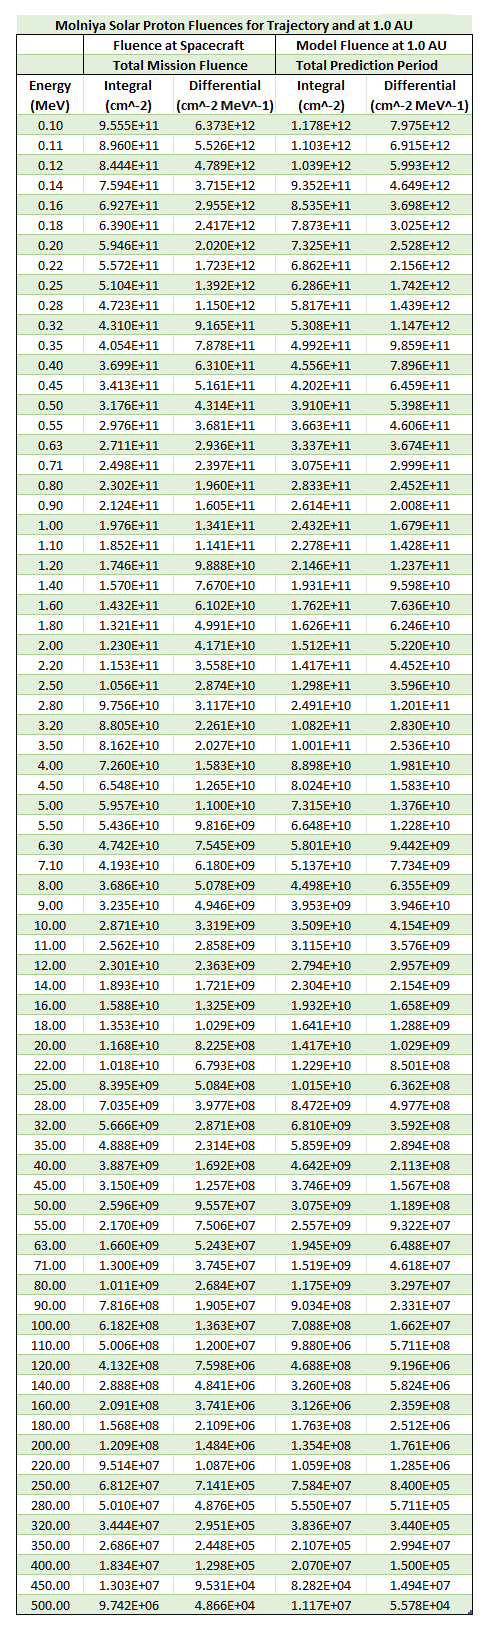
\includegraphics[width=0.78\linewidth]{Molniya_SP.png}
        \caption{The Molniya Solar Particle Emission Spectrum.}
        \label{fig:MolniyaSP}
    \end{minipage}
\end{figure}

\begin{figure}[H]
    \centering
        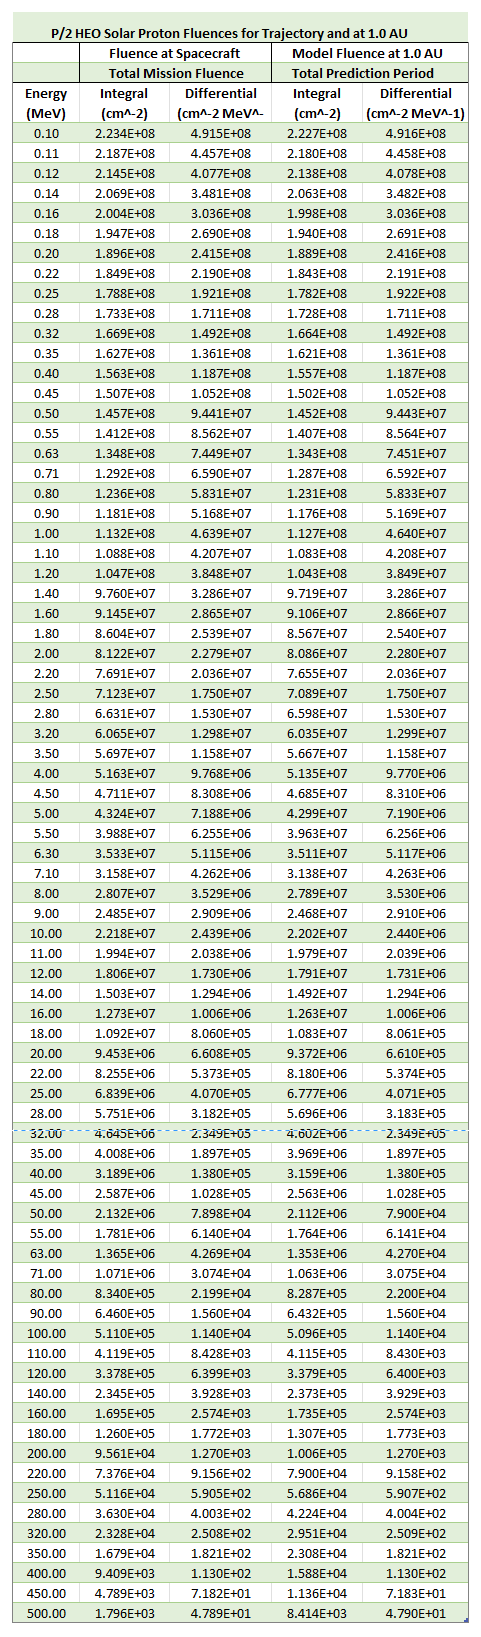
\includegraphics[width=0.40\linewidth]{TESS_SP.png}
        \caption{The P/2 HEO Solar Particle Emission Spectrum.}
        \label{fig:TESSSP}
\end{figure}

\begin{figure}[H]
    \centering
        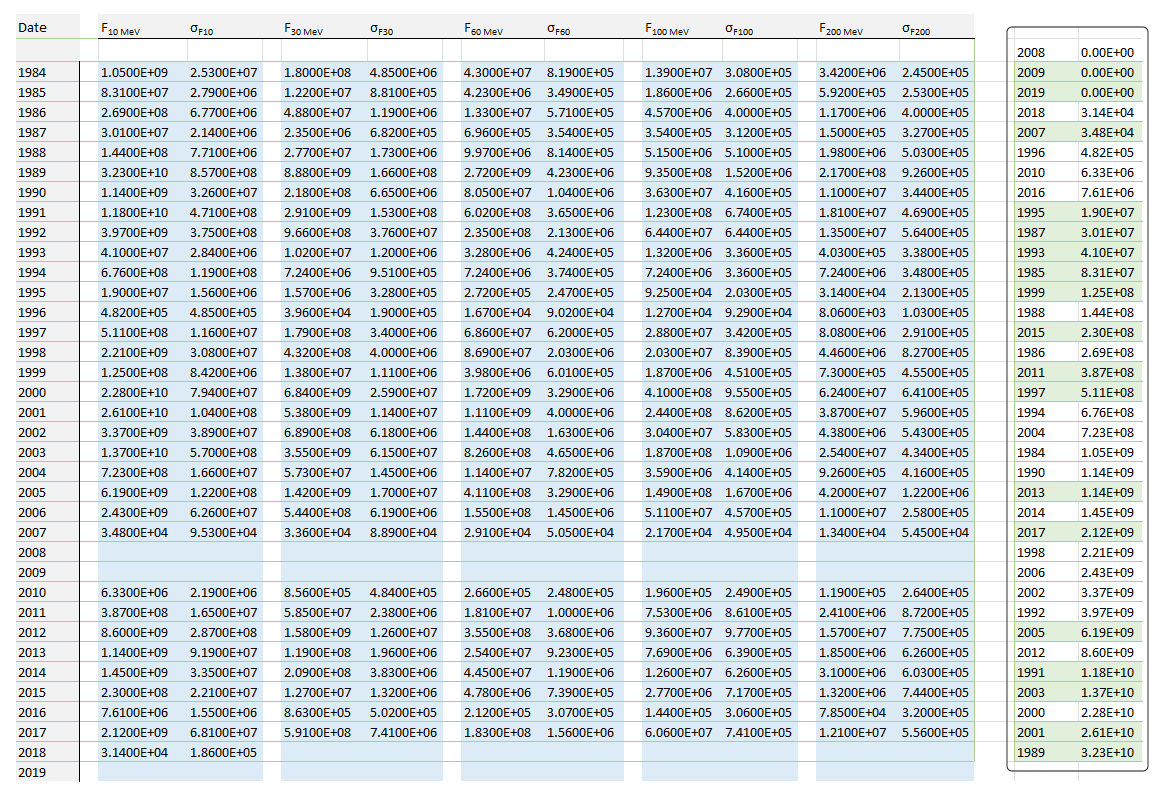
\includegraphics[width=1\linewidth]{ETO_Events.png}
        \caption{The Earth Trailing Orbit radiation exposure data. The values are total yearly fluence, along with error, for each energy bin. Bins start at the expressed value and continue to the next bin's value. The first bin is therefore $ 10 \leq x < 30 $  Mev. }
        \label{fig:ETORad}
\end{figure}

\section{Radiation Comparisons}
The following charts show comparisons of orbital radiation data. Blue regions indicate integral trapped particle fluences; orange shading indicates differential trapped particle fluences; green shading indicates comparisons. 

The 'Difference' columns indicate the multiplier difference between the P/2 HEO orbit and the MEO and Molniya orbits, with the P/2 being the primary orbit that the others are compared to:

\[ \frac{F_{Comp} - F_{HEO}}{F_{Comp}} \]

A negative sign in these columns indicates that the P/2 HEO receives a \textit{lower} exposure than the comparison orbit in that energy range. For example, in Figure~\ref{fig:COMPTrapped}, in the 0.50 MeV bin, in the first green column, the value indicates that the P/2 orbit receives 14,500 times less fluence in that energy bin than does the MEO orbit. 

\subsection{Trapped Particle Fluence Comparison}

The trapped particle fluence comparison chart is shown in Figure~\ref{fig:COMPTrapped}. Cells with 'F=0' values indicate that there is no significant fluence in that energy bin. An empty cell means that the P/2 orbit has reached zero while the comparison orbit has not.

\begin{figure}[!t]
    \centering
        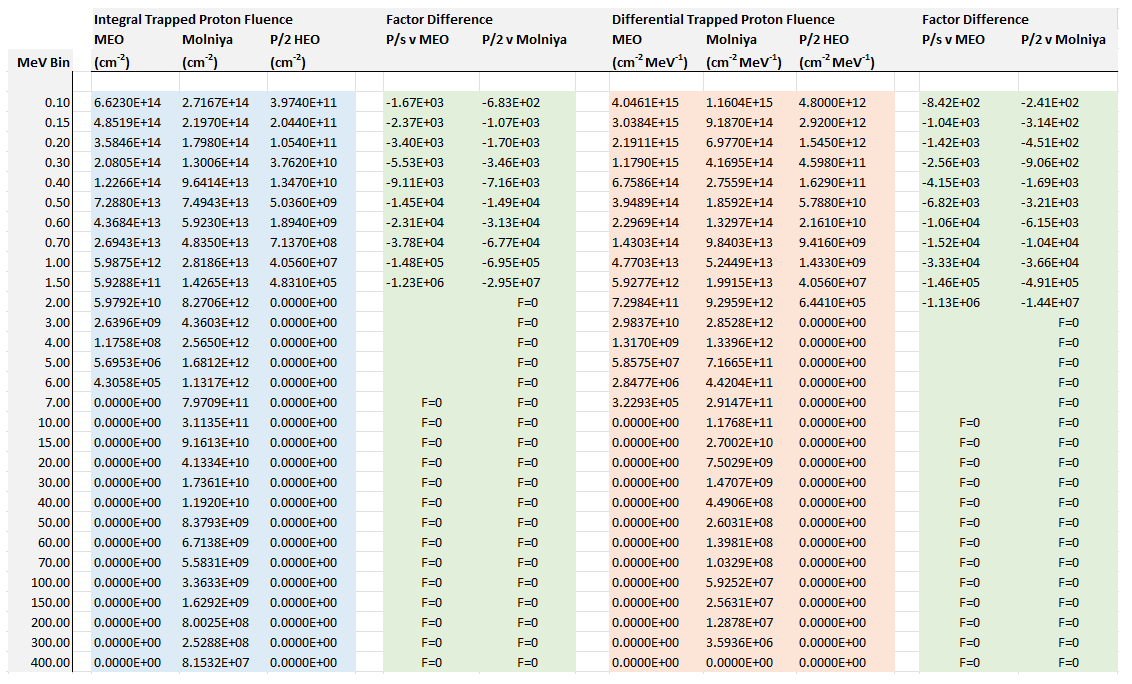
\includegraphics[width=1\linewidth]{COMP_Trapped.png}
        \caption{Comparison of the fluence values of the P/2 HEO orbit to the MEO and Molniya orbits. A negative sign indicates that the P/2 is exposed to less trapped particle fluence by the given multiplier. A cell value of 'F=0' indicates that there is no fluence from that range of particle energies.}
        \label{fig:COMPTrapped}
\end{figure}

\subsection{Solar Proton Fluence Comparison}

The solar proton fluence comparison chart is shown in Figure~\ref{fig:COMPSolar}. The relative scarcity of ETO data points, and the energy value mismatch at several of those points, limits the P/2 HEO comparison significantly.

\begin{figure}
    \centering
        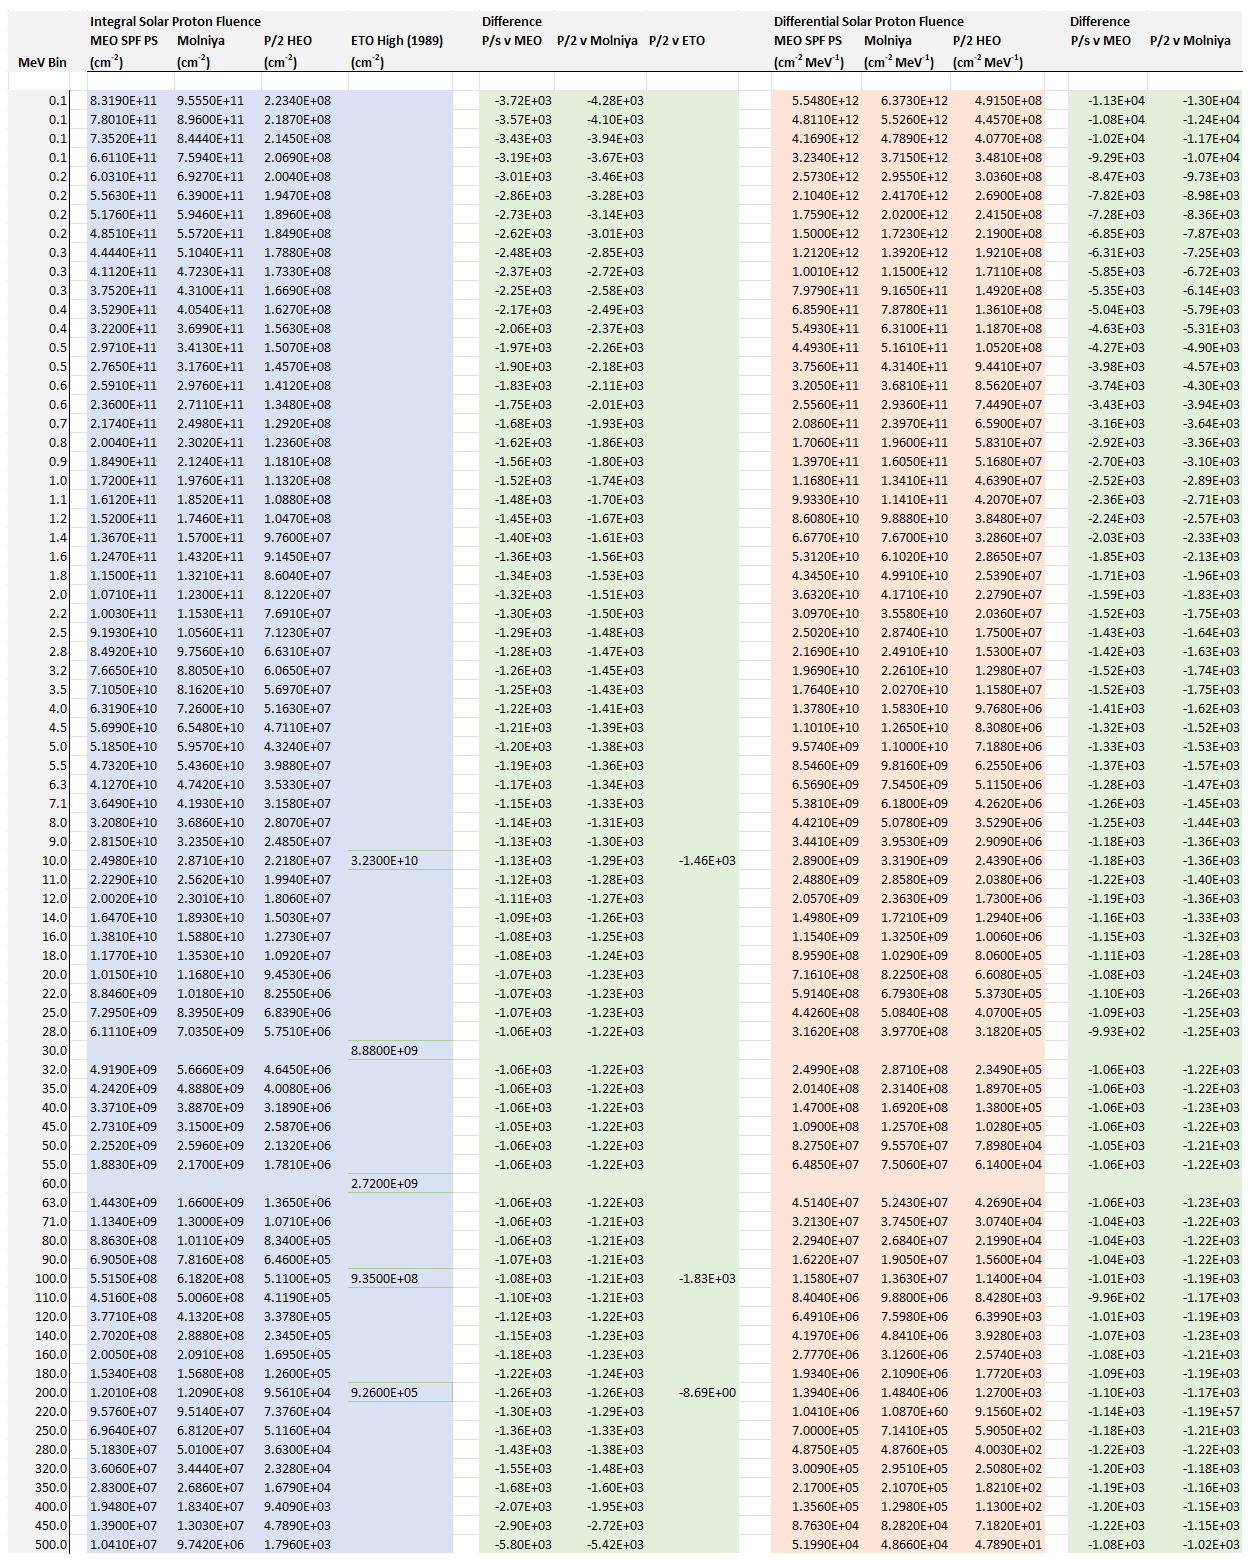
\includegraphics[width=1\linewidth]{COMP_Solar.png}
        \caption{Comparison of the solar proton fluence values of the P/2 HEO orbit to the MEO and Molniya orbits. A negative sign indicates that the P/2 is exposed to less solar proton fluence by the given multiplier. A cell value of 'F=0' indicates that there is no fluence from that range of particle energies.}
        \label{fig:COMPSolar}
\end{figure}

\section{Conclusions}

The purpose of this brief paper is to compare the proton fluence results for a one-year segment of a mission on each of four orbits under consideration. Proton fluences for three of the orbits, the MEO, the Molniya and the P/s HEO, were generated by SPENVIS, using the considerations discussed in Section~\ref{sec:notes}. Fluences for the ETO orbit were the results of in situ measurements taken by the NOAA GEOS-R satellites, as discussed in Section~\ref{sec:GEOS}.

\subsection{Trapped Particle Exposure}

As noted in the previous sections, the MEO and Molniya orbits have considerable intersection with both the proton and electron regions of the Van Allen belts, while the P/2 HEO in its science orbit has no intersection. We would expect to see this reflected in the trapped particle fluences, and we do. 

The MEO (and EMEO) orbit intersects the outer region of the proton belts, and so is exposed to mostly lower energy protons. This is reflected in its proton spectra by its proton fluence dropping to zero at around 7.0 MeV. However, a glance at the intersection image shows that both the MEO and the EMEO orbits intersect the region of the \textit{highest} energy electron belts. The loss of high energy proton fluence is countered by the gain in high energy electron fluence.

Whereas the MEO and EMEO orbits are constantly immersed in the belts, the Molniya's intersection occurs for a small portion of its orbit, on the approach and departure from perigee, but it is still enough to crank its fluence levels to fairly high levels. During the time it passes through its two mirror image exposures, it manages to pass through all energy level zones of both protons and electrons, and this is reflected by having relatively high fluence values across its entire spectrum.

Given that the P/2 avoids the belts entirely during its science trajectory, its only exposures to belt particles is during the initial phasing orbits (which is not included in these calculations), and in the science orbit when it is exposed to the cloud of low energy particles that get distributed outwards from the belt as a result of the solar wind. (This affects the Molniya orbit as well.)

\vspace{0.5cm}

\textbf{Conclusion:} \textit{The P/2 orbit receives significantly lower high energy trapped proton and electron fluence, by as much as seven orders of magnitude, across all energy bins, than does the MEO, EMEO, or Molniya orbits.} 

\subsection{Solar Proton Exposure}

Similarly, in terms of high energy solar proton fluence, the P/2 also receives significantly less fluence across all energy bins then does the MEO or Molniya orbit. And, perhaps not surprisingly, given the ETO orbit's position outside of the magnetosphere, the P/2 also receives less fluence then does the ETO orbit, although admittedly comparison data points for the ETO are limited.

\vspace{0.5cm}

\textbf{Conclusion:} \textit{The P/2 orbit receives significantly lower high energy solar proton fluence, by three orders of magnitude, across all energy bins, than does the MEO, EMEO, or Molniya orbits.} 

\subsection{Summary}

None of this is actually surprising, given several factors. The P/2 orbit is a masterpiece of orbital design, and was specifically engineered to avoid the Van Allen belts, reducing its exposure to trapped particle fluence. But it remains comfortably inside the magnetosphere, reducing its exposure to solar protons. 

Given the other considerations the designers took into consideration, such as the precise countering of solar and lunar perturbances to create a highly stable orbit and the reduction of orbital eclipsing, the low radiation profile of the P/2 orbit is yet another reason to recommend the P/2 Highly Elliptical Orbit.

\newpage
\appendix
\appendixpage
\addappheadtotoc

\section{Table of Solar Proton Events}

A problem with adopting an Earth Trailing Orbit is that missions under consideration utilize off-the shelf components for mission-critical instruments. These components are not radiation hardened. The ETO orbit is constantly  exposed to solar proton events, and is therefore at the mercy of constant bombardment by high energy solar protons and the unpredictability of major solar events. 

I have included tables reprinted from Raukunen and Usoskin's 2022 article \textit{Annual integral solar proton fluences for 1984-2019} as a reminder of the extreme variability in solar proton events. A glance through Figures~\ref{fig:SP01} and~\ref{fig:SP02} show the extreme output that these solar discharges produce. 

\begin{figure}[H]
    \centering
        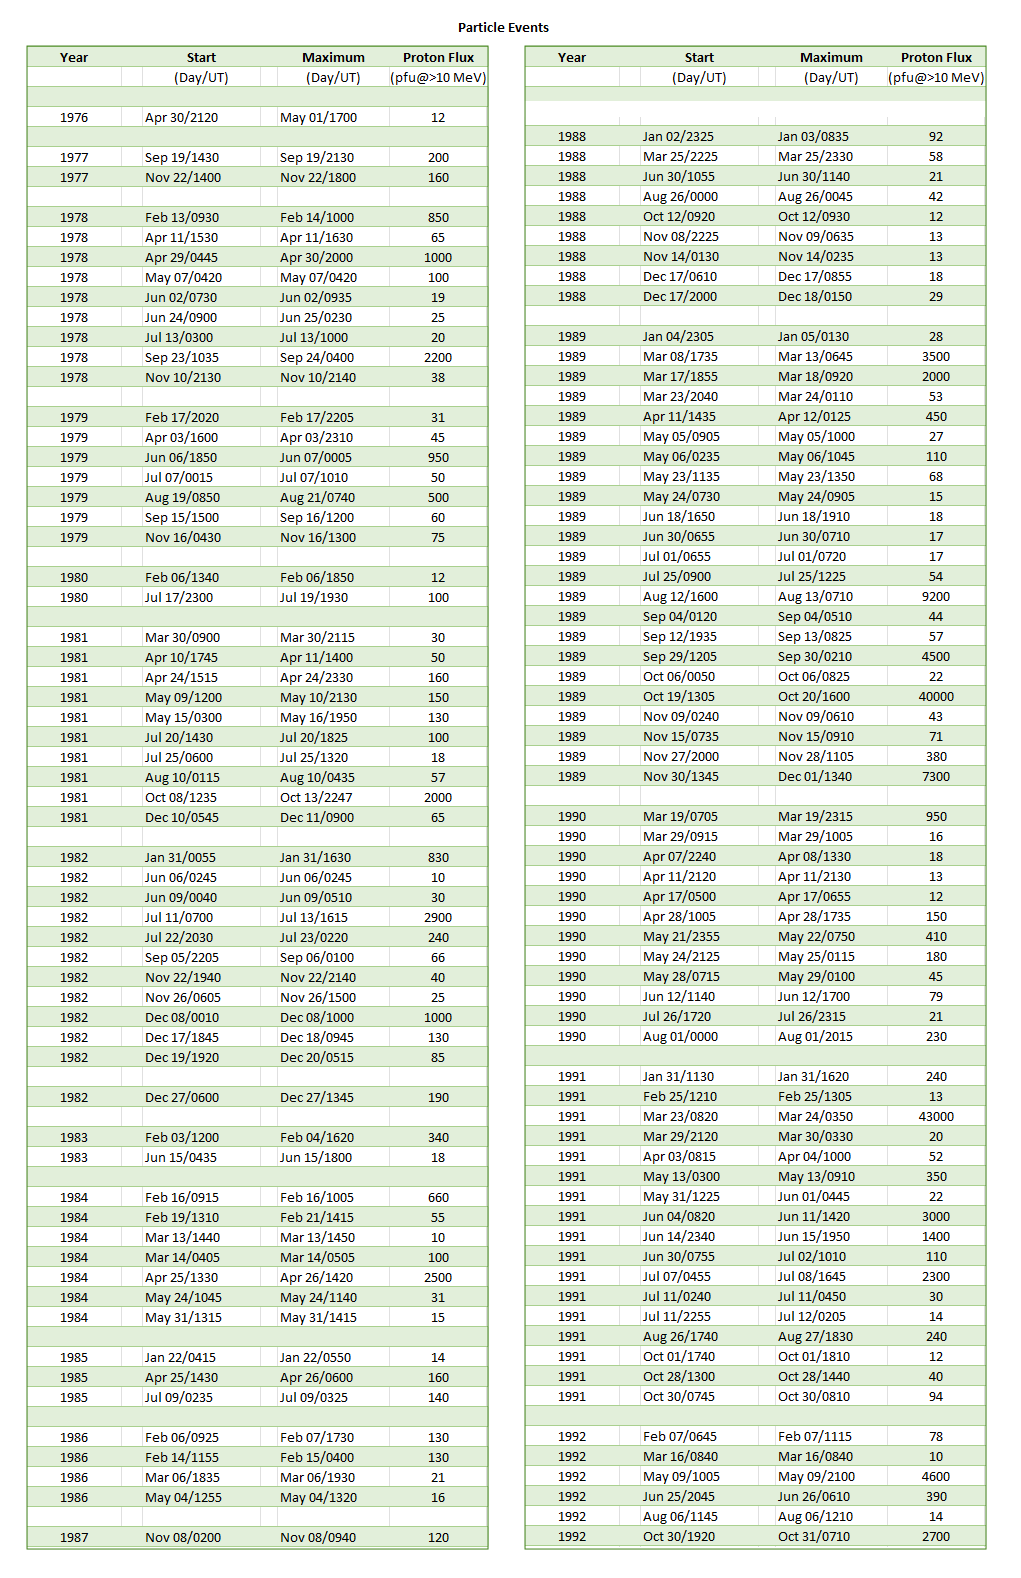
\includegraphics[width=.86\linewidth]{SolarFlareEvents01.png}
        \caption{Table of Solar Flare Proton Events, 1976-1992.}
        \label{fig:SP01}
\end{figure}

\begin{figure}[H]
    \centering
        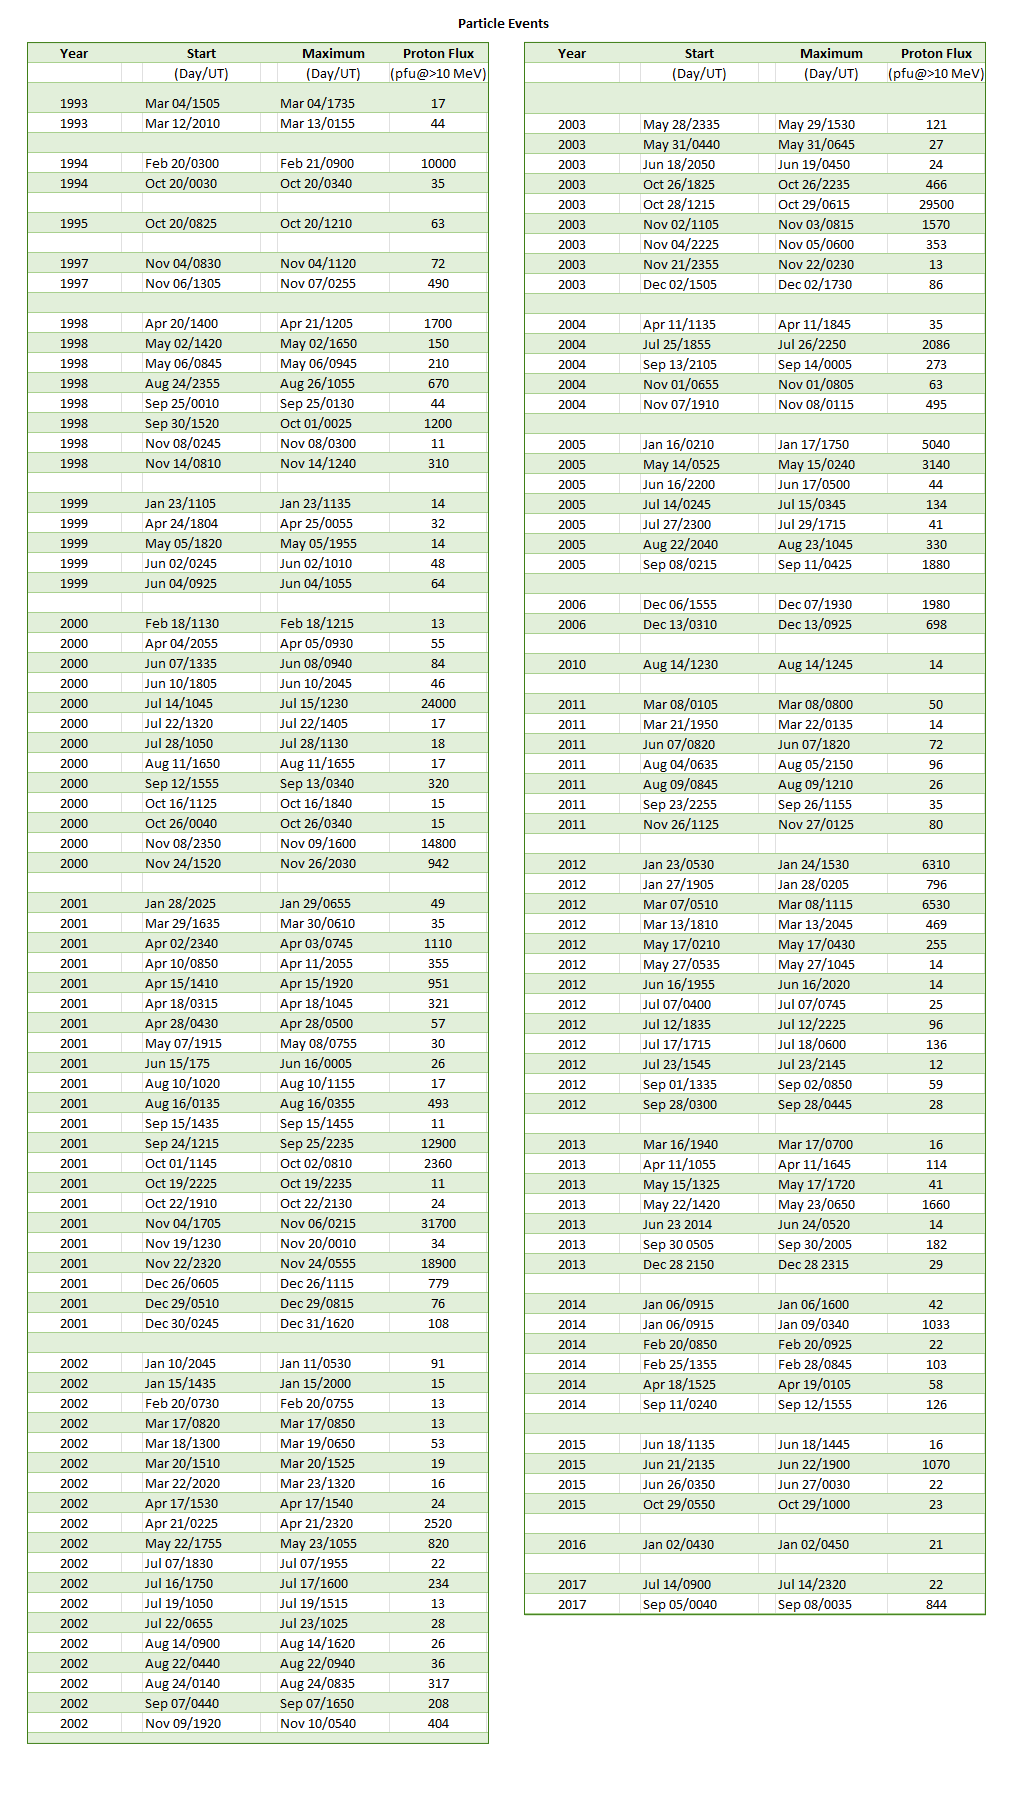
\includegraphics[width=.75\linewidth]{SolarFlareEvents02.png}
        \caption{Table of Solar Flare Proton Events, 1993-2017.}
        \label{fig:SP02}
\end{figure}

% Bibliography --------------------------------------------------------------------

\defbibnote{myprenote}{Note: All illustrations and tables created by author.}
\printbibliography[prenote=myprenote]

\end{document}